\documentclass[leqno, openany]{memoir}
\setulmarginsandblock{3.5cm}{3.5cm}{*}
\setlrmarginsandblock{3cm}{3.5cm}{*}
\checkandfixthelayout

\usepackage{amsmath}
\usepackage{amssymb}
\usepackage{amsthm}
%\usepackage{MnSymbol}
\usepackage{bm}
\usepackage{accents}
\usepackage{mathtools}
\usepackage{tikz}
\usetikzlibrary{calc}
\usetikzlibrary{automata,positioning}
\usepackage{tikz-cd}
\usepackage{forest}
\usepackage{braket} 
\usepackage{listings}
\usepackage{mdframed}
\usepackage{verbatim}
\usepackage{physics2}
\usephysicsmodule{ab,ab.legacy,diagmat,xmat}
\usepackage{derivative}
\usepackage{fixdif}
\usepackage{stmaryrd}
\usepackage{mathrsfs} 
\usepackage[normalem]{ulem} 
\usepackage{stackengine}
\usepackage{bbm}
%\usepackage{/home/patrickl/homework/macaulay2}

%font
\usepackage[sc]{mathpazo}
\usepackage{eucal}
\usepackage[scaled=0.86]{berasans}
\usepackage{inconsolata}
\usepackage{microtype}

%CS packages
\usepackage{algorithmicx}
\usepackage{algpseudocode}
\usepackage{algorithm}

% typeset and bib
\usepackage[english]{babel} 
\usepackage[utf8]{inputenc} 
\usepackage[T1]{fontenc}
\usepackage[bookmarks, colorlinks, breaklinks]{hyperref} 
\hypersetup{linkcolor=blue,citecolor=magenta,filecolor=black,urlcolor=blue}
\usepackage{cleveref}
\usepackage[backend=biber,style=alphabetic,maxalphanames=4,maxnames=5,hyperref,backref=true,backrefstyle=none]{biblatex}
\usepackage{xpatch}
\xpatchbibmacro{pageref}{parens}{backrefparens}{}{}
\crefname{equation}{}{}

% other formatting packages
\usepackage{float}
\usepackage{booktabs}
\usepackage[shortlabels]{enumitem}
\usepackage{csquotes}
\usepackage{titlesec}
\usepackage{titling}
\usepackage{parskip}
\usepackage{graphicx}
\graphicspath{{./}}

\usepackage{lipsum}

% delimiters
\DeclarePairedDelimiter{\gen}{\langle}{\rangle}
\DeclarePairedDelimiter{\floor}{\lfloor}{\rfloor}
\DeclarePairedDelimiter{\ceil}{\lceil}{\rceil}


\newtheorem{thm}{Theorem}[section]
\newtheorem{cor}[thm]{Corollary}
\newtheorem{prop}[thm]{Proposition}
\newtheorem{lem}[thm]{Lemma}
\newtheorem{conj}[thm]{Conjecture}
\newtheorem{quest}[thm]{Question}
\newtheorem{prob}[thm]{Problem}

\theoremstyle{definition}
\newtheorem{defn}[thm]{Definition}
\newtheorem{defns}[thm]{Definitions}
\newtheorem{con}[thm]{Construction}
\newtheorem{exm}[thm]{Example}
\newtheorem{exms}[thm]{Examples}
\newtheorem{notn}[thm]{Notation}
\newtheorem{notns}[thm]{Notations}
\newtheorem{addm}[thm]{Addendum}
\newtheorem{exer}[thm]{Exercise}

\theoremstyle{remark}
\newtheorem{rmk}[thm]{Remark}
\newtheorem{rmks}[thm]{Remarks}
\newtheorem{warn}[thm]{Warning}
\newtheorem{sch}[thm]{Scholium}


% unnumbered theorems
\theoremstyle{plain}
\newtheorem*{thm*}{Theorem}
\newtheorem*{prop*}{Proposition}
\newtheorem*{lem*}{Lemma}
\newtheorem*{cor*}{Corollary}
\newtheorem*{conj*}{Conjecture}

% unnumbered definitions
\theoremstyle{definition}
\newtheorem*{defn*}{Definition}
\newtheorem*{exer*}{Exercise}
\newtheorem*{defns*}{Definitions}
\newtheorem*{con*}{Construction}
\newtheorem*{exm*}{Example}
\newtheorem*{exms*}{Examples}
\newtheorem*{notn*}{Notation}
\newtheorem*{notns*}{Notations}
\newtheorem*{addm*}{Addendum}


\theoremstyle{remark}
\newtheorem*{rmk*}{Remark}

% shortcuts
\newcommand{\Ima}{\mathrm{Im}}
\newcommand{\A}{\mathbb{A}}
\newcommand{\F}{\mathbb{F}}
\newcommand{\E}{\mathcal{E}}
\newcommand{\G}{\mathbb{G}}
\newcommand{\N}{\mathbb{N}}
\newcommand{\R}{\mathbb{R}}
\newcommand{\C}{\mathbb{C}}
\newcommand{\Z}{\mathbb{Z}}
\newcommand{\Q}{\mathbb{Q}}
\newcommand{\bS}{\mathbb{S}}
\renewcommand{\k}{\Bbbk}
\renewcommand{\L}{\mathbb{L}}
\renewcommand{\P}{\mathbb{P}}
\newcommand{\M}{\overline{M}}
\newcommand{\g}{\mathfrak{g}}
\newcommand{\h}{\mathfrak{h}}
\newcommand{\n}{\mathfrak{n}}
\renewcommand{\b}{\mathfrak{b}}
\newcommand{\ep}{\varepsilon}
\newcommand*{\dt}[1]{%
   \accentset{\mbox{\Huge\bfseries .}}{#1}}
\renewcommand{\abstractname}{Official Description}
\newcommand{\mc}[1]{\mathcal{#1}}
\newcommand{\T}{\mathbb{T}}
\newcommand{\mf}[1]{\mathfrak{#1}}
\newcommand{\mr}[1]{\mathrm{#1}}
\newcommand{\ms}[1]{\mathsf{#1}}
\newcommand{\mt}[1]{\mathtt{#1}}
\newcommand{\mbf}[1]{\mathbf{#1}}
\newcommand{\mb}[1]{\mathbb{#1}}
\newcommand{\on}[1]{\operatorname{#1}}
\newcommand{\ol}[1]{\overline{#1}}
\newcommand{\ul}[1]{\underline{#1}}
\newcommand{\wt}[1]{\widetilde{#1}}
\newcommand{\wh}[1]{\widehat{#1}}
\renewcommand{\div}{\operatorname{div}}
\newcommand{\bir}{\sim_{\mr{bir}}}
\newcommand{\vir}{\mr{vir}}
\newcommand{\stacks}[1]{\href{https://stacks.math.columbia.edu/tag/#1}{#1}}
\newcommand{\ostar}{\stackMath\mathbin{\stackinset{c}{0ex}{c}{0ex}{\star}{\bigcirc}}}
\newcommand{\Mbar}{\overline{\mathcal{M}}}

\DeclareMathOperator{\Der}{Der}
\DeclareMathOperator{\Def}{Def}
\DeclareMathOperator{\Bl}{Bl}
\DeclareMathOperator{\NE}{NE}
\DeclareMathOperator{\Tor}{Tor}
\DeclareMathOperator{\Hom}{Hom}
\DeclareMathOperator{\Ext}{Ext}
\DeclareMathOperator{\End}{End}
\DeclareMathOperator{\ad}{ad}
\DeclareMathOperator{\Aut}{Aut}
\DeclareMathOperator{\Rad}{Rad}
\DeclareMathOperator{\Pic}{Pic}
\DeclareMathOperator{\supp}{supp}
\DeclareMathOperator{\Supp}{Supp}
\DeclareMathOperator{\sgn}{sgn}
\DeclareMathOperator{\spec}{Spec}
\DeclareMathOperator{\Spec}{Spec}
\DeclareMathOperator{\proj}{Proj}
\DeclareMathOperator{\Proj}{Proj}
\DeclareMathOperator{\ord}{ord}
\DeclareMathOperator{\Div}{Div}
\DeclareMathOperator{\depth}{depth}
\DeclareMathOperator{\coker}{coker}
\DeclareMathOperator{\codim}{codim}
\DeclareMathOperator{\ch}{ch}
\DeclareMathOperator{\ev}{ev}
\DeclareMathOperator{\Hilb}{Hilb}
\DeclareMathOperator{\QDM}{QDM}

% Section formatting
\titleformat{\section}
    {\Large\sffamily\scshape\bfseries}{\thesection}{1em}{}
\titleformat{\subsection}[runin]
    {\large\sffamily\bfseries}{\thesubsection}{1em}{}
\titleformat{\subsubsection}[runin]{\normalfont\itshape}{\thesubsubsection}{1em}{}

\title{COURSE TITLE}
\author{Lectures by INSTRUCTOR, Notes by NOTETAKER}
\date{SEMESTER}

\newcommand*{\titleSW}
    {\begingroup% Story of Writing
    \raggedleft
    \vspace*{\baselineskip}
    {\Huge\itshape Enumerative invariants and birational geometry\\ Spring 2024}\\[\baselineskip]
    {\large\itshape Notes by Patrick Lei}\\[0.2\textheight]
    {\Large Lectures by Various}\par
    \vfill
    {\Large \sffamily Columbia University}
    \vspace*{\baselineskip}
\endgroup}
\pagestyle{simple}

\chapterstyle{ell}


%\renewcommand{\cftchapterpagefont}{}
\renewcommand\cftchapterfont{\sffamily}
\renewcommand\cftsectionfont{\scshape}
\renewcommand*{\cftchapterleader}{}
\renewcommand*{\cftsectionleader}{}
\renewcommand*{\cftsubsectionleader}{}
\renewcommand*{\cftchapterformatpnum}[1]{~\textbullet~#1}
\renewcommand*{\cftsectionformatpnum}[1]{~\textbullet~#1}
\renewcommand*{\cftsubsectionformatpnum}[1]{~\textbullet~#1}
\renewcommand{\cftchapterafterpnum}{\cftparfillskip}
\renewcommand{\cftsectionafterpnum}{\cftparfillskip}
\renewcommand{\cftsubsectionafterpnum}{\cftparfillskip}
\setrmarg{3.55em plus 1fil}
\setsecnumdepth{subsection}
\maxsecnumdepth{subsection}
\settocdepth{subsection}

\addbibresource{../../math.bib}
\DefineBibliographyStrings{english}{
    backrefpage={$\leftarrow$},
    backrefpages={$\leftarrow$},
}

\begin{document}
    
\begin{titlingpage}
\titleSW
\end{titlingpage}

\thispagestyle{empty}
\section*{Disclaimer}%
\label{sec:disclaimer}

These notes were taken during the lectures using \texttt{neovim}. 
Any errors are mine and not the speakers'. 
In addition, my notes are picture-free (but will include commutative diagrams) and are a mix of my mathematical style and that of the lecturers. Also, notation may differe between lecturers.
If you find any errors, please contact me at \texttt{plei@math.columbia.edu}.

\section*{Acknowledgements}
I would like to thank Shaoyun Bai for co-organizing the seminar with me.

\vspace*{1cm}

\noindent\textbf{Seminar Website:}  \url{https://math.columbia.edu/~plei/s24-birat.html}
\newpage

\tableofcontents

\chapter{Preliminaries}%
\label{cha:Preliminaries}

\section{Givental formalism (Patrick, Feb 01)}

\subsection{Introduction}

Let $X$ be a smooth projective variety. Then for any $g,n \in \Z_{\geq 0}, \beta \in H_2(X,\Z)$, there exists a moduli space $\Mbar_{g,n}(X,\beta)$ (Givental's notation is $X_{g,n,\beta}$) of \textit{stable maps} $f \colon C \to X$ from genus-$g$, $n$-marked prestable curves to $X$ with $f_*[C] = \beta$. It is well-known that $\Mbar_{g,n}(X,\beta)$ has a virtual fundamental class
\[ [\Mbar_{g,n}(X,\beta)]^{\mr{vir}} \in A_{\delta}(\Mbar_{g,n}(X,\beta)), \qquad \delta = \int_{\beta} c_1(X) + (\dim X - 3)(1-g) + 3. \]
In addition, there is a universal curve and sections
\begin{equation*}
\begin{tikzcd}
    \mc{C} \ar[shift left=1]{r}{\pi} & \Mbar_{g,n}(X,\beta) \ar[shift left=1]{l}{\sigma_i}.
\end{tikzcd}
\end{equation*}
In this setup, there are tautological classes
\[ \psi_i \coloneqq c_1(\sigma_i^* \omega_{\pi}) \in H^2(\Mbar_{g,n}(X,\beta)). \]
This allows us to define individual Gromov-Witten invariants by
\[ \ab<\tau_{a_1}(\phi_1) \cdots \tau_{a_n}(\phi_n)>_{g,n,\beta}^X = \int_{[\Mbar_{g,n}(X,\beta)]^{\mr{vir}}} \prod_{i=1}^n \on{ev}_i^* \phi_i \cdot \psi_i^{a_i}. \]
These invariants satisfy various relations. The first is the \textit{string equation:}
\[ \ab<\tau_0(1) \tau_{a_1}(\phi_1) \cdots \tau_{a_n}(\phi_n)>_{g,n+1,\beta}^X = \sum_{i=1}^n \ab<\tau_{a_i-1}(\phi_i)\prod_{j\neq i} \tau_{a_j}(\phi_j)>_{g,n,\beta}^X. \]
The next is the \textit{dilaton equation:}
\[ \ab<\tau_1(1) \tau_{a_1}(\phi_1) \cdots \tau_{a_n}(\phi_n)>_{g,n+1,\beta}^X = (2g-2+n)\ab<\tau_{a_1}(\phi_1) \cdots \tau_{a_n}(\phi_n)>_{g,n,\beta}^X. \]
Finally, we have the \textit{divisor equation} when one insertion is a divisor $D \in H^2(X)$:
\begin{align*}
    \ab<\tau_0(D)\tau_{a_1}(\phi_1)\cdots \tau_{a_n}(\phi_n)>_{g,n+1,\beta}^X =&{} \ab(\int_{\beta} D) \cdot \ab<\tau_{a_1}(\phi_1) \cdots \tau_{a_n}(\phi_n)>_{g,n,\beta}^X \\
    &+ \sum_{i=1}^n \ab<\tau_{a_i-1}(\phi_i \cdot D)\prod_{j\neq i} \tau_{a_j}(\phi_j)>_{g,n,\beta}^X.
\end{align*}

It is often useful to package Gromov-Witten invariants into various generating series.

\begin{defn}
    The \textit{quantum cohomology} $QH^*(X)$ of $X$ is defined by the formula
    \[ (a \star_t b, c) \coloneqq \sum_{\beta, n} \frac{Q^{\beta}}{n!} \ab<a,b,c,t,\ldots,t>_{0,3+n,\beta}^X \]
    for any $t \in H^*(X)$. This is a commutative and associative product.
\end{defn}
The \textit{small quantum cohomology} is obtained by setting $t=0$ and the ordinary cohomology is obtained by further setting $Q=0$.
\begin{rmk}
    Convergence of the formula does not hold in general, so quantum cohomology needs to be treated as a formal object.
\end{rmk}

\begin{defn}\label{defn:jfunction}
    Let $\phi_i$ be a basis of $H^*(X)$ and $\phi^i$ be the dual basis. Then the \textit{$J$-function} of $X$ is the cohomology-valued function
    \[ J_X(t,z) \coloneqq z + t + \sum_i \sum_{n,\beta} \frac{Q^{\beta}}{n!} \ab<\frac{\phi_i}{z-\psi}, t, \ldots, t>_{0,n+1,\beta}^X \phi^i. \]
\end{defn}

\begin{defn}
    The \textit{genus-$0$ GW potential} of $X$ is the (formal) function
    \[ \mc{F}^X(t(z)) = \sum_{\beta, n} \frac{Q^{\beta}}{n!} \ab<t(\psi), \ldots, t(\psi)>_{0,n,\beta}^X. \]
\end{defn}

The associativity of the quantum product is equivalent to the PDE
\[ \sum_{e,f} \mc{F}^X_{abe} \eta^{ef} \mc{F}_{cdf} = \sum_{e,f} \mc{F}^X_{ade} \eta^{ef} \mc{F}^X_{bcf} \]
for any $a,b,c,d$, which are known as the \textit{WDVV equations}. Here, we choose coordinates on $H^*(X)$ and set $z=0$ (only consider primary insertions). In addition, set $\eta_{ef}$ to be the components of the Poincar\'e pairing and let $\eta^{ef}$ be the inverse matrix.


\subsection{Frobenius manifolds}

A Frobenius manifold can be thought of as a formalization of the WDVV equations.

\begin{defn}
    A \textit{Frobenius manifold} is a complex manifold $M$ with a flat symmetric bilinear form $\ab<-,->$ (meaning that the Levi-Civita connection has zero curvature) on $TM$ and a holomorphic system of (commutative, associative) products $\star_t$ on $T_t M$ satisfying:
    \begin{enumerate}
        \item The unit vector field $\mbf{1}$ is flat: $\nabla \mbf{1} = 0$;
        \item For any $t$ and $a,b,c \in T_t M$, $\ab<a \star_t b, c> = \ab<a, b \star_t c>$;
        \item If $c(u,v,w) \coloneqq \ab<u \star_t v, w>$, then the tensor $(\nabla_z c)(u,v,w)$ is symmetric in $u,v,w,z \in T_t M$.
    \end{enumerate}
    If there exists a vector field $E$ such that $\nabla \nabla E = 0$ and complex number $d$ such that:
    \begin{enumerate}
        \item $\nabla \nabla E = 0$;
        \item $\mc{L}_E(u \star v) - \mc{L}_E u \star v - u \star \mc{L}_E v = u \star v$ for all vector fields $u,v$;
        \item $\mc{L}_E \ab<u,v> - \ab<\mc{L}_E u,v> - \ab<u,\mc{L}_E v> = (2-d) \ab<u,v>$ for all vector fields $u,v$,
    \end{enumerate}
    then $E$ is called an \textit{Euler vector field} and the Frobenius manifold $M$ is called \textit{conformal}.
\end{defn}

\begin{exm}
    Let $X$ be a smooth projective variety. Then we can give $H^*(X)$ the structure of a Frobenius algebra with the Poincar\'e pairing and the quantum product. Note that the quantum product does not converge in general, so we must treat this as a formal object. The Euler vector field is given by
    \[ E_X = c_1(X) + \sum_i \ab(1-\frac{\deg \phi_i}{2})t^i \phi_i, \]
    where a general element of $H^*(X)$ is given by $t = \sum_i t^i \phi_i$. We will also impose that $\phi_1 = \mbf{1}$. There is another very important structure, the \textit{quantum connection}, which is given by the formula
    \begin{align*}
        \nabla_{t^i} &\coloneqq \partial_{t^i} + \frac{1}{z} \phi_i \star_t \\
        \nabla_{z \odv{}{z}} &\coloneqq z \odv{}{z} - \frac{1}{z} E_X \star_t + \mu_X.
    \end{align*}
    Here, $\mu_X$ is the \textit{grading operator}, defined for pure degree classes $\phi \in H^*(X)$ by
    \[ \mu_X(\phi) = \frac{\deg \phi - \dim X}{2} \phi. \]
    Finally, in the direction of the Novikov variables, we have
    \[ \nabla_{\xi Q \partial_Q} = \xi Q \partial_Q + \frac{1}{z} \xi \star_t. \]
\end{exm}

\begin{rmk}
    For a general conformal Frobenius manifold $(H, (-,-), \star, E)$, there is still a \textit{deformed flat connection} or \textit{Dubrovin connection} given by
    \begin{align*}
        \nabla_{t^i} &\coloneqq \pdv{}{t^i} + \frac{1}{z} \phi_i \star \\
        \nabla_{z \odv{}{z}} &\coloneqq z \odv{}{z} - \frac{1}{z} E \star.
    \end{align*}
\end{rmk}


\begin{defn}
    The \textit{quantum $D$-module} of $X$ is the module $H^*(X)[z]\llbracket Q,t\rrbracket$ with the quantum connection defined above.
\end{defn}

\begin{rmk}
    It is important to note that the quantum connection has a fundamental solution matrix $S^X(t,z)$ given by
    \[ S_X(t,z) \phi = \phi + \sum_{i} \sum_{n,\beta} \frac{Q^{\beta}}{n!} \phi^i \ab<\frac{\phi_i}{z-\psi},\phi,t,\ldots,t>_{0,n+2,\beta}^X. \]
    It satisfies the important equation
    \[ S_X^*(t,-z) S(t,z) = 1. \]
    Using this formalism, the $J$-function is given by $S_X^*(t,z) \mbf{1} = z^{-1} J_X(t,z)$.
\end{rmk}


\subsection{Givental formalism}

The Givental formalism is a geometric way to package enumerative (CohFT) invariants cleanly. We begin by defining the symplectic space
\[ \mc{H} \coloneqq H^*(X, \Lambda)\llparenthesis z^{-1}\rrparenthesis \]
with the symplectic form
\[ \Omega(f,g) \coloneqq \on{Res}_{z=0} ( f(-z)g(z) ). \]
This has a polarization by Lagrangian subspaces
\[ \mc{H}_+ \coloneqq H^*(X,\Lambda)[z], \qquad \mc{H}_- \coloneqq z^{-1} H^*(X,\Lambda)\llbracket z^{-1} \rrbracket \]
giving $\mc{H} \cong T^* \mc{H}_+$ as symplectic vector spaces. Choose Darboux coordinates $\ul{p}, \ul{q}$ on $\mc{H}$. For example, there is a choice in Coates's thesis which gives a general element of $\mc{H}$ as
\[ \sum_{k \geq 0} \sum_i q_k^i \phi_i z^k + \sum_{\ell \geq 0} \sum_j p_{\ell}^j \phi^j (-z)^{-\ell-1}. \]

Taking the \textit{dilaton shift}
\[ q(z) = t(z) - z = -z + t_0 + t_1 z + t_2 z^2 + \cdots, \]
we can now think of $\mc{F}^X$ has a formal function on $\mc{H}_+$ near $q = -z$. This convention is called the \textit{dilaton shift}.

Before we continue, we need to recast the string and dilaton equations in terms of $\mc{F}^X$. Write $t_x = \sum t_k^i \phi_i$. Then the string equation becomes
\[ \partial_0^1 \mc{F}(t) = \frac{1}{2} (t_0, t_0) + \sum_{n=0}^{\infty} \sum_{j} t_{n+1}^{j} \partial_n^{j} \mc{F}(t) \]
and the dilaton equation becomes
\[ \partial_1^1 \mc{F}(t) = \sum_{n=0}^{\infty} t_n^j \partial_n^j \mc{F}(t) - 2 \mc{F}(t). \]
There are also an infinite series of topological recursion relations
\[ \partial_{k+1}^i \partial_{\ell}^j \partial_{m}^k \mc{F}(t) = \sum_{a,b} \partial_k^i \partial_0^a \mc{F}(t) \eta^{ab} \partial_0^b \partial_{\ell}^j \partial_m^k \mc{F}(t). \]
We can make sense of these three relations for any (formal) function $\mc{F}$ on $\mc{H}_+$.

Now let
\[ \mc{L} = \ab\{(\ul{p}, \ul{q}) \in \mc{H} \mid \ul{p} = \d_{\ul{q}} \mc{F}\} \]
be the graph of $\d \mc{F}$. This is a formal germ at $q=-z$ of a Lagrangian section of the cotangent bundle $T^* \mc{H}_+$ and is therefore a formal germ of a Lagrangian submanifold in $\mc{H}$.

\begin{thm}\label{thm:overruled}
    The function $\mc{F}$ satisfies the string equation, dilaton equation, and topological recursion relations if and only if $\mc{L}$ is a Lagrangian cone with vertex at the origin $q=0$ such that its tangent spaces $L$ are tangent to $\mc{L}$ exactly along $z L$.
\end{thm}

Because of this theorem, $\mc{L}$ is known as the \textit{Lagrangian cone}. It can be recovered from the $J$-function by the following procedure. First consider $\mc{L} \cap (-z + z \mc{H}_-)$. Via the projection to $-z + H$ along $\mc{H}_-$, this can be considered as the graph of the $J$-function. Next, we consider the derivatives $\pdv{J}{t^i}$, which form a basis of $L \cap z \mc{H}_-$, which is a complement to $zL$ in $L$. Then we know that
\[ z \pdv{J}{t^i} \in z L \subset \mc{L}, \]
so 
\[ z \pdv{J}{t^i,t^j} \in L \cap z \mc{H}_-. \]
Writing these in terms of the first derivatives $\pdv{J}{t^i}$ and using the fact that $J$ is a solution of the quantum connection, so we recover the Frobenius structure of quantum cohomology.

We will now express some classical results in this formalism. Let $X$ be a toric variety with toric divisors $D_1, \ldots, D_N$ such that $D_1, \ldots, D_k$ form a basis of $H^2(X)$ and Picard rank $k$. Then define the \textit{$I$-function}
\[ I_X = z e^{\sum_{j=1}^k t_i D_i} \sum_{\beta} Q^{\beta} \frac{\prod_{j=1}^N \prod_{m=-\infty}^0 (D_j+mz)}{\prod_{j=1}^N \prod_{m=-\infty}^{\ab<D_j, \beta>}(D_j + mz)}. \]

\begin{thm}[Mirror theorem]
    The formal functions $I_X$ and $J_X$ coincide up to some change of variables, which if $c_1(X)$ is semi-positive is given by components of the $I$-function.
\end{thm}


\begin{thm}[Mirror theorem in this formalism]
    For any $t$, we have
    \[ I_X(t, z) \in \mc{L}. \]
\end{thm}

Another direction in Gromov-Witten theory is the Virasoro constraints. In the original formulation, these involved very complicated explicit differential operators, but in the Givental formalism, there is a very compact formulation.

Define $\ell^{-1} = z^{-1}$ and
\[ \ell_0 = z \odv{}{z} + \frac{1}{2} + \mu + \frac{c_1(X) \cup -}{z}. \]
Then define 
\[ \ell_n = \ell_0 (z \ell_0)^n. \]

\begin{thm}[Genus-$0$ Virasoro constraints]
    Suppose the vector field on $\mc{H}$ defined by $\ell_0$ is tangent to $\mc{L}$. Then the same is true for the vector fields defined by $\ell_n$ for any $n \geq 1$.
\end{thm}

\begin{proof}
    Let $L$ be a tangent space to $\mc{L}$. Then if $f \in zL \subset \mc{L}$, the assumption gives us $\ell_0 f \in L$. But then $z \ell_0 f \in zL$, so $\ell_0 z \ell_0 f = \ell_1 f \in L$. Continuing, we obtain $\ell_n f \in L$ for all $n$.
\end{proof}

Later, we will learn that the Quantum Riemann-Roch theorem can be stated in this formalism. Let $\mc{L}^{\mr{tw}}$ be the twisted Lagrangian cone (where the twisted theory will be defined next week).
\begin{thm}[Quantum Riemann-Roch]
    For some explicit linear symplectic transformaiton $\Delta$, we have $\mc{L}^{\mr{tw}} = \Delta \mc{L}$.
\end{thm}




\subsection{Quantization}

In the last part of the talk, we will briefly discuss the quantization formalism, which encodes the higher-genus theory. In Darboux coordinates $p_a, q_b$, we will quantize symplectic transformations by the standard rules
\[ \wh{{q_a q_b}} = \frac{q_a q_b}{\hslash}, \qquad \wh{q_a p_b} = q_a \pdv{}{q_b}, \qquad \wh{p_a p_b} = \hslash \pdv{}{q_a,q_b}. \]
This determines a differential operator acting on functions on $\mc{H}_+$.

We also need the genus-$g$ potential
\[ \mc{F}_g^X \coloneqq \sum_{\beta, n} \frac{Q^{\beta}}{n!} \ab<t(\psi), \ldots, t(\psi)>_{g,n,\beta}^X \]
and the \textit{total descendent potential}
\[ \mc{D} \coloneqq \exp\ab(\sum_{g \geq 0} \hslash^{g-1} \mc{F}_g^X). \]

In this formalism, the Virasoro conjecture can be expressed as follows. Let $L_n = \wh{\ell}_n + c_n$, where $c_n$ is a carefully chosen constant.

\begin{conj}[Virasoro conjecture]
    If $L_{-1} \mc{D} = L_0 \mc{D} = 0$, then $L_n \mc{D} = 0$ for all $n \geq 1$.
\end{conj}

In this formalism, the higher-genus version of the Quantum Riemann-Roch theorem takes the very simple form
\begin{thm}[Quantum Riemann-Roch]
    Let $\mc{D}^{\mr{tw}}$ be the twisted descendent potential. Then
    \[ \mc{D}^{\mr{tw}} = \wh{\Delta} \mc{D}. \]
\end{thm}

\section{Quantum Riemann-Roch (Shaoyun, Feb 08)}

We will state and prove the Quantum Riemann-Roch theorem in genus $0$, following Coates-Givental.

\subsection{Twisted Gromov-Witten invariants}

Again, let $X$ be a smooth projective variety. Let $E$ be a vector bundle on $X$. We should note that 
\[ \Mbar_{0,n+1}(X,\beta) \xrightarrow{\pi} \Mbar_{0,n}(X,\beta) \]
is the universal curve, and the universal morphism is simply $\on{ev}_{n+1}$. We will consider the sheaf
\[ E_{0,n,\beta} \coloneqq R\pi_* \on{ev}_{n+1}^* E \in K^0(\Mbar_{0,n}(X, \beta)). \]
We need to check that this is a well-defined $K$-theory class. Choose an ample line bundle $L \to X$. By definition, for $N \gg 1$, the cohomology
\[ H^i(X, E \otimes L^N) = 0 \]
whenever $i \geq 1$. This gives us an exact sequence
\[ 0 \to \ker ( \eqqcolon A ) \to H^0(X, E \otimes L^N) \otimes L^{-N} ( \eqqcolon B ) \to E \to 0. \]
For any stable map $f \colon \Sigma \to X$ of positive degree, we obtain a long exact sequence
\begin{equation*}
    0 \to H^0(\Sigma, f^* E) \to H^1(\Sigma, f^* A) \to H^1(\Sigma, f^* B) \to H^1(\Sigma, f^* E) \to 0,
\end{equation*}
so we obtain
\[ R^0 \pi_* \ev_{n+1}^* E - R^1 \pi_* \ev_{n+1}^* E = R^1 \pi_* \ev_{n+1}^* B - R^1 \pi_* \ev_{n+1}^* A. \]
This expresses $E_{0,n,\beta}$ as a difference of vector bundles.

We will now introduce a \textit{universal characteristic class}
\[ \mbf{c}(-) = \exp \ab( \sum_{k=0}^{\infty} s_k \ch_k(-)), \]
where $s_0, s_1, s_2, \ldots$ are formal variables and $\ch_k$ is the $k$-th Chern character
\[ \frac{x_1^k}{k!} + \cdots + \frac{x_r^k}{k!}, \]
where $x_i$ are the Chern roots.

\begin{exm}
    Let $E \to X$ be a vector bundle and equip it with the fiberwise $\C^*$-action by scaling. Let $\lambda$ be the equivariant parameter and $\rho_i$ be the Chern roots. Then
    \[ e(E) = \sum_i (\lambda + \rho_i). \]
    We then rewrite
    \begin{align*}
        \prod( \lambda + \rho_i) &= \exp\ab(\sum_i \ab(\log \lambda - \sum_k \frac{(-\rho_i)^k}{k\lambda^k})) \\
        &= \exp\ab(\ch_0(E) \log \lambda + \sum_{k > 0} \frac{(-1)^{k-1}(k-1)!}{\lambda^k} \ch_k(E)),
    \end{align*}
    so for the (equivariant Euler class), we obtain
    \begin{align*}
        s_0 &= \log \lambda \\
        s_k &= \frac{(-1)^{k-1} (k-1)!}{\lambda^k}, \qquad k > 0.
    \end{align*}
\end{exm}

We are now ready to define the $(E,\mbf{c})$-twisted Gromov-Witten invariants.

\begin{defn}
    Define the \textit{twisted Gromov-Witten invariants} by
    \[ \ab<\alpha_1 \psi_1^{k_1}, \ldots, \alpha_n \psi_n^{k_n}>_{0,n,\beta}^{X,(E, \mbf{c})} \coloneqq \int_{[\Mbar_{0,n}(X,\beta)]^{\mr{vir}}} \prod_{i=1}^n \ev_i^*(\alpha_i)\psi_i^{k_i} \cup \mbf{c}(E_{0,n,\beta}) \]
    for $\alpha_i \in H^*(X)$ and $k_i \in \Z_{\geq 0}$.
\end{defn}

We will now construct the Lagrangian cone for the twisted theory. Let $R$ be the coefficient ring containing $s_0, s_1, \ldots$ and define
\[ \mc{H}^{\mr{tw}}_X \coloneqq H^*(X)\otimes R\llparenthesis z^{-1}\rrparenthesis \llbracket Q \rrbracket. \]
We also introduce the \textit{twisted Poincar\'e pairing}
\[ (a,b)_{(E, \mbf{c})} = \int_X a \cup b \cup \mbf{c}(E). \]
The symplectic structure is defined by
\[ \Omega_{\mr{tw}}(f,g) = \on{Res}_{z=0} (f(-z) g(z))_{(E,\mbf{c})}. \]
There is a polarization
\[ \mc{H}^{\mr{tw}}_X = \mc{H}_+^{\mr{tw}} \oplus \mc{H}_-^{\mr{tw}} \]
with
\begin{align*}
    \mc{H}_+^{\mr{tw}} &\coloneqq H^*(X) \otimes R[z]\llbracket Q \rrbracket \\
    \mc{H}_-^{\mr{tw}} &\coloneqq H^*(X) \otimes R\llbracket z\rrbracket\llbracket Q \rrbracket.
\end{align*}
Finally, we have the \textit{twisted genus-$0$ descendent potential}
\[ \mc{F}_{X,\mr{tw}}^0(t) \coloneqq \sum_{\beta, n} \frac{Q^{\beta}}{n!} \ab<t,\ldots,t>_{0,n,\beta}^{X,(E,\mbf{c})}. \]
Identifying $\mc{H}^{\mr{tw}}_X$ with $T^* \mc{H}_+^{\mr{tw}}$, we obtain the twisted Lagrangian cone $\mc{L}_X^{\mr{tw}}$ as the graph of $\d \mc{F}^0_{X,\mr{tw}}$. Denote the untwisted Lagrangian cone as $\mc{L}_X$.

\begin{thm}\label{thm:qrr}
    We have
    \[ \mc{L}_X^{\mr{tw}} = \Delta \mc{L}_X, \]
    where
    \[ \Delta = \exp\ab(\sum_{m \geq 0} \sum_{\ell \geq 0} s_{2m-1+\ell} \frac{B_{2m}}{(2m)!} \ch_{\ell}(E) z^{2m-1}). \]
    Here, the Bernoulli numbers $B_{2m}$ are defined by
    \[ \frac{t}{1-e^{-t}} = \frac{t}{2} + \sum_{m \geq 0} \frac{B_{2m}}{(2m!)} t^{2m}. \]
\end{thm}

\subsection{Proof of~\Cref{thm:qrr}}

The idea is to use the Grothendieck-Riemann-Roch theorem.

\begin{prop}
    We can write
    \[ [\Mbar_{0,n}(X,\beta)]^{\vir} \cap \ch_k(E_{0,n,\beta}) = \pi_* \ab(\sum_{\substack{r+\ell=k+1 \\ r,\ell \geq 0}} \frac{B_r}{r!} \ch_{\ell}(\ev^*_{n+1} E) \Psi(r)), \]
    where
    \begin{align*}
        \Psi(r) ={}& \psi_{n+1}^r \cap [\Mbar_{0,n+1}(X,\beta)]^{\vir} \\ 
        &- \sum_{i=1}^n (\sigma_i)_* (\psi_i^{n-1} \cap [\Mbar_{0,n}(X,\beta)]^{\vir}) \\ 
        &+ \frac{1}{2} j_* \ab(\sum_{\substack{a+b=r-2 \\ a,b \geq 0}} (-1)^a \psi_+^a \psi_i^b \cap [\wt{Z}_{0,n+1,\beta}]^{\vir}). 
    \end{align*}
    Here, $Z_{0,n+1,\beta}$ is formed by the nodes of $\pi$, $\wt{Z}_{0,n+1,\beta}$ is a double cover of $Z_{0,n+1,\beta}$ formed by a choice of branch of the nodes,  $\psi_+$ and $\psi_-$ are the $\psi$-classes at the two branches of the nodes, and
    \[ j \colon \wt{Z}_{0,n+1,\beta} \to Z_{0,n+1,\beta} \to \Mbar_{0,n+1}(X,\beta) \]
    is the ``inclusion.''
\end{prop}

\begin{proof}
    We will first assume that $\ol{M}_{0,n+1}(X,\beta)$, $\Mbar_{0,n}(X,\beta)$, and $Z_{0,n+1,\beta}$ are all smooth and that $\pi(Z_{0,n+1,\beta})$ is a normal crossings divisor. In general, we need a Cartesian diagram
    \begin{equation*}
    \begin{tikzcd}
        & \ev_{n+1}^* E \ar{rr} \ar{dl} & & E \ar{dl} \\
        \Mbar_{0,n+1}(X,\beta) \ar{rr} \ar{dd} & & \mc{C} \ar{dd} \\
        & Z_{0,n+1,\beta} \ar[hookrightarrow]{ul} & & Z \ar[hookrightarrow]{ul} \\
        \Mbar_{0,n}(X,\beta) \ar{rr} & & \mc{M}.
    \end{tikzcd}
    \end{equation*}
    Continuing in the ideal situation, we apply Grothendieck-Riemann-Roch\footnote{We need to be careful about directly applying Grothendieck-Riemann-Roch in the stacky setting (and in general we are only quasi-smooth).} to obtain
    \begin{align*}
        \ch(E_{0,n,\beta}) &= \ch(R \pi_* \ev_{n+1}^* E) \\
        &= \pi_* (\ch(\ev_{n+1}^* E) \cdot \on{td}^{\vee} \Omega_{\pi}),
    \end{align*}
    where $\on{td}^{\vee}$ is the dual Todd class, defined by $\frac{-x}{1-e^{tx}}$, and $\Omega_{\pi}$ is the sheaf of relative differentials.

    We then have two short exact sequences
    \[ 0 \to \Omega_{\pi} \to \omega_{\pi} \to \mc{O}_{Z_{0,n+1,\beta}} \to 0 \]
    and
    \[ 0 \to \omega_{\pi} \to L_{n+1} \to \bigoplus_{i=1}^n \mc{O}_{D_i} \to 0, \]
    where $D_i$ is the divisor where the marked points $i, n+1$ collide and their component has exactly three special points. Now we obtain
    \[ \Omega_{\pi} = L_{n+1} - \sum_{i=1}^n \mc{O}_{D_i} - \mc{O}_{Z_{0,n+1,\beta}} \]
    in $K$-theory. Using the facts that $c_1(L_{n+1}) = \psi_{n+1}$, $D_i \cap D_j = \emptyset$ for $i \neq j$, and $D_i \cap Z_{0,n+1,\beta} = \emptyset$, we see that $L_{n+1}$ is trivial when restricted to $D_i$ and $Z_{0,n+1,\beta}$. Now we apply the dual Todd class.
    \begin{lem}
        If $x_1 \cup x_2 = 0$, then
        \[ (\on{td}^{\vee}(x_1)-1)(\on{td}^{\vee}(x_2)-1) = 0. \]
    \end{lem}
    Using the lemma, we obtain
    \begin{align*}
        \on{td}^{\vee}(\Omega_{\pi}) &= \on{td}^{\vee}(L_{n+1}) \prod_{i=1}^n \on{td}^{\vee}(-\mc{O}_{D_i}) \on{td}^{\vee}(\mc{O}_{Z_{0,n+1,\beta}})^{-1} \\
        &= 1 + (\on{td}^{\vee}(L_{n+1})-1) + \sum_{i=1}^n\ab(  \frac{1}{\on{td}^{\vee}(\mc{O}_{D_i})} -1 ) + \ab(\frac{1}{\on{td}^{\vee}(\mc{O}_{Z_{n+1,\beta}})}-1).
    \end{align*}
    The first term in the statement comes from the dual Todd class of $L_{n+1}$, the second comes from
    \[ 0 \to \mc{O}(-D_i) \to \mc{O} \to \mc{O}_{D_i} \to 0 \]
    and the relation between $\mc{O}(-D_i)$ and $L_i$, and the last term can be found in Appendix A of Coates-Givental.
\end{proof}

To obtain the Quantum Riemann-Roch theorem, we use the previous proposition and manipulate the generating function. If $E$ is convex and $Y \subset X$ is a complete intersection defined by $E$, then $\mc{L}_X^{\mr{tw}}$ is closely related to $\mc{L}_Y$, so we are able to study the Gromov-Witten theory of $Y$ using this.

\section{Shift operators (Melissa, Feb 15)}%
\label{sec:shift_operators}

Let $X$ be a semiprojective smooth variety. This means that $X$ is projective over its affinization. Also assume that $X$ has an action by $T = (\C^{\times})^m$ such that all $T$-weights in $H^0(X, \mc{O})$ are contained in a strictly convex cone in $\Hom(T, \C^{\times})_{\R}$ and $H^0(X, \mc{O})^T = \C$. All such $X$ imply that
\begin{enumerate}[(a)]
    \item The fixed locus $X^T$ is projective;
    \item The $T$-variety $X$ is equivariantly formal. This means that $H_T^*(X)$ is a free module over $H_T^*(\mr{pt}) = \Q[\lambda] \coloneqq \Q[\lambda_1, \ldots, \lambda_m]$ and there is a non-canonical isomorphism
        \[ H_T^*(X) \cong H^*(X) \otimes H_T^*(\mr{pt}) \]
        as $H_T^*(\mr{pt})$-modules.
    \item The evaluation maps $\on{ev}_i \colon X_{0,n,d} \to X$ are proper.
\end{enumerate}
Using (b), we may choose a basis $\ab\{\phi_i\}_{i=0}^N$ of $H_T^*(X)$ over $H_T^*(\mr{pt})$. Let $\tau^i$ be the dual coordinates.

\subsection{Equivariant big quantum cohomology}%
\label{sub:Equivariant big quantum cohomology}
Let $(-,-)$ be the $T$-equivariant Poincar\'e pairing, which in general takes values in $\Q(\lambda)$. Then the $T$-equivariant big quantum product is defined by
\begin{align*}
    (\phi_i \star_{\tau} \phi_j, \phi_k) &= \ab<\!\! \ab< \phi_i, \phi_j, \phi_k>\!\!>_{0,3}^{X,T} \\
    &= \sum_{d,n} \frac{Q^d}{n!} \ab<\phi_i, \phi_b, \phi_j,\tau, \ldots, \tau>_{0,n+3,d}^{X,T}. 
\end{align*}
This can also be defined using the evaluation maps
\[ (\on{ev}_i)_* \colon H_T^*(X_{0,n+3,d}) \to H_T^{*-2(c_1(X) \cdot d + n)}(X) \]
as
\[ \phi_i \star_{\tau} \phi_j = \sum_{d,n} \frac{Q^d}{n!} (\on{ev}_3)_* \ab(\ev_1^*(\phi_i) \ev_2^*(\phi_j) \prod_{i=4}^{n+3} \ev_i^*(\tau) \cap [X_{0,n+3,d}]^{\vir}) \in H_T^*(X)\llbracket Q \rrbracket \llbracket\tau_0,\ldots,\tau_n\rrbracket. \]

\subsection{Quantum connection}%
\label{sub:Quantum connection}

We will define
\[ \nabla_i \colon H_T^*(X)[z] \llbracket Q \rrbracket \llbracket\tau\rrbracket \to z^{-1} H_T^*(X)[z] \llbracket Q \rrbracket \llbracket\tau^0, \ldots, \tau^N\rrbracket \]
by setting
\[ \nabla_i = \pdv{}{\tau^i} + \frac{1}{z} (\phi_i \star). \]
We can view $z$ as the loop variable by setting $\wh{T} = T \times \C^{\times}$. If the extra copy of $\C^{\times}$ acts trivially on $X$, then
\[ H_{\wh{T}}^*(X) = H_T^*(X)[z]. \]
This has a fundamental solution
\[ M(\tau) \colon H_{\wh{T}}^*(X) \llbracket Q, \tau \rrbracket \to H_{\wh{T}}^*(X)_{\mr{loc}} \llbracket Q, \tau \rrbracket \]
where
\[ H_{\wh{T}}^*(X)_{\mr{loc}} \coloneqq H_{\wh{T}}^*(X) \otimes_{\Q[\lambda,z]} \Q(\lambda(z)). \]
This satisfies the differential equation
\[ z \pdv{}{\tau^i} M(\tau) = M(\tau) (\phi_i \star), \]
which is equivalent to
\[ \pdv{}{\tau^i} \circ M(\tau) = M(\tau) \circ \nabla_i. \]
The solution has the form
\[ (M(\tau) \phi_i, \phi_j) = (\phi_i, \phi_j) + \ab<\!\!\! \ab< \phi_i, \frac{\phi_j}{z-\psi}>\!\!\!>_{0,2}^{X,T}. \]

\subsection{Shift operators}%
\label{sub:Shift operators}

Let $k \colon \C^{\times} \to T$ be a cocharacter of $T$. Then define a $\wh{T}$-action $\rho_k$ on $X$ by
\[ \rho_k(t,x) x = t u^k \cdot x \]
for $t \in T, u \in \C^{\times}, x \in X$. Under the group automorphism
\[ \phi_k \colon \wh{T} \to \wh{T} \qquad \phi_k(t,u) = (tu^{-k}, u), \]
the identity map $(X, \rho_0) \to (X, \rho_k)$ is $\wh{T}$-equivariant, so we obtain isomorphisms
\[ \Phi_k \colon H_{\wh{T}, \rho_0}^*(X) \to H_{\wh{T}, \rho_k}^*(X). \]

Now define the bundle
\[ E_k = (X \times (\C^2 \setminus 0)) / \C^{\times}, \]
where $\C^{\times}$ acts by
\[ s \cdot (x, v_1, v_2) = (s^k x, s^{-1}v_1, s^{-1} v_2). \]
This is an $X$-bundle over $\P^1$ with an action on $\wh{T}$ by
\[ (t,u) \cdot [x, (v_1, v_2)] = [t \cdot x, (v_1, u v_2)]. \]
Setting $0 = [1,0]$ and $\infty = [0,1]$, we see that $\wh{T}$ acts on $X_0$ by $\rho_0$ and $X_{\infty}$ by $\rho_k$.

\begin{defn}
    A cocharacter $k \colon \C^{\times} \to T$ is \textit{seminegative} if all weights of $H^0(X, \mc{O})$ are nonpositive with respect to $k$ and is \textit{negative} if all nonzero weights of $H^0(X, \mc{O})$ are negative.
\end{defn}

\begin{lem}
    If $k$ is seminegative, then $E_k$ is semiprojective.
\end{lem}

Now let $\pi \colon E_k \to \P^1$ be the projection. We now consider \textit{section classes}, which are those effective classes in $H_2(E_k, \Z)$ satisfying $\pi_* d = [\P^1]$. For the $\C^{\times}$-action on $X$ given by $k$, there is a unique fixed component $F_{\mr{min}}$ whose normal weights are all positive (one way to see this is to consider the moment map of the corresponding circle action). Therefore, there is a minimal section class $\sigma_{\min}$ corresponding to $F_{\min}$.

\begin{lem}
    Given $\tau \in H_T^*(X)$, there exists $\wh{\tau} \in H_{\wh{T}}^*(E_k)$ such that $\wh{\tau}|_{X_0} = \tau$ and $\wh{\tau}|_{X_{\infty}} = \Phi_k(\tau)$.
\end{lem}


\begin{lem}
    If $k$ is seminegative, then
    \[ \on{Eff}(E_k)^{\mr{sec}} = \sigma_{\min} + \on{Eff}(X). \]
\end{lem}

\begin{defn}
    Let $k \colon \C^{\times} \to T$ be seminegative. Given $\tau \in H_T^*(X)$, we define the \textit{shift operator} 
    \[ \wt{\mathbb{S}}_k \colon H_{\wh{T}, \rho_0}^*(X) \llbracket Q \rrbracket \to H_{\wh{T}, \rho_k}^*(X) \llbracket Q \rrbracket \] 
    by the formula
    \[ (\wt{\mathbb{S}}_k(\tau) \alpha, \beta) = \sum_{\wh{d} \in \on{Eff}(E_k)^{\mr{sec}}} \frac{Q^{\wh{d} - \sigma_{\min}}}{n!} \ab< (\iota_0)_* \alpha, (\iota_{\infty})_* \beta, \wh{\tau}, \ldots, \wh{\tau}>_{0,n+2,\wh{d}}^{E_k, \wh{T}}, \]
    where $\alpha \in H_{\wh{t}, \rho_0}^*(X)$ and $\beta \in H_{\wh{T}, \rho_k}^*(X)$. We also define
    \[ \bS_k(\tau) = \Phi_k^{-1} \circ \wh{\bS}_k(\tau). \]
\end{defn}

\begin{thm}
    We have the formula
    \[ M(\tau) \circ \bS_k(\tau) = \mc{S}_k \circ M(\tau), \]
    where $\mc{S}_k$ is defined via the commutative diagram
    \begin{equation*}
    \begin{tikzcd}
        H_{\wh{T}}^*(X)_{\mr{loc}} \ar{rr}{\mc{S}_k} \ar{d} & & H_{\wh{T}}^*(X)_{\mr{loc}} \ar{d}{\iota^*} \\
        H_{\wh{T}}^*(X^T)_{\mr{loc}} \ar{rr}{\bigoplus_i \Delta_i(k) e^{-2k\delta_{\lambda}}} & & H_{\wh{T}}^*(X^T)_{\mr{loc}}.
    \end{tikzcd}
    \end{equation*}
    Here, we define
    \[ \Delta_i(k) = Q^{\sigma_i - \sigma_{\min}} \prod_{\alpha} \prod_{j=1}^{\on{rk} N_{i,\alpha}} \frac{\prod_{c=-\infty}^0 (\rho_{i,\alpha,j} + \alpha + cz)}{\prod_{c=-\infty}^{-\alpha \cdot k} (\rho_{i,\alpha,j} + \alpha + cz)} \in H_{\wh{T}}^*(F_i)_{\mr{loc}} \llbracket Q \rrbracket, \]
    where 
    \[ N_i = N_{F_i/X} = \bigoplus_{\alpha} N_{i,\alpha} \]
    is the normal bundle of $F_i$ in $X$ and $\rho_{i,\alpha,j}$ are its Chern roots.
\end{thm}

The idea of the proof is to decompose
\[ E_{k,0,n+2,\wh{d}}^{\wh{T}} = \bigsqcup_i \bigsqcup_{I_1 \cup I_2 = [n+2]} \bigsqcup_{d_0 + d_{\infty} + \wh{\sigma} = \wh{{d}}} (X_0)_{0,I_1 \sqcup p, d_0}^T \times_{F_i} (X_{\infty})_{0,I_2 \sqcup q, d_{\infty}}^T. \]
Using the exact sequence
\[ 0 \to \Aut(C,x) \to \on{Def}(f) \to T^1 \to \on{Def}(C,x) \to \on{Obs}(f) \to T^2 \to 0, \]
we obtain the explicit formulae
\begin{align*}
    \Aut(C,x)^m &= \Aut(C_0,x_0)^m + \Aut(C_{\infty}, x_{\infty})^m \\
    \on{Def}(C,x)^m &= \on{Def}(C_0, x_0)^m \oplus \on{Def}(C_0, x_0)^m \oplus T_p C_0 \otimes T_p \P^1 \oplus T_q C_{\infty} \otimes T_q \P^1.
\end{align*}
This gives the virtual normal bundle, and using virtual localization, we obtain
\[ (\wt{\bS}_k(\tau) \alpha, \beta) = (\wt{\mc{S}}_k M(\tau, z) \alpha, M'(\tau', -z) \beta), \]
where
\[ M'(\tau', z) = \Phi_k \circ M(\tau, z) \circ \Phi_k^{-1}. \]
Using the unitarity property of $M$, we obtain the desired result.

\chapter{Quantum cohomology of projective bundles}%
\label{cha:Quantum cohomology of projective bundles}

\section{Mirror theorem (Che, Feb 22)}%
\label{sec:Mirror theorem}

\subsection{Setup}%
\label{sub:Setup}

Let $X$ be a smooth projective variety, $\ab\{ \phi_i\}_{i=0}^s$ be a basis of $H^*(X)$, $\ab\{\phi^i\}_{i=0}^s$ be the dual basis, and 
\[ \tau = \sum_{i=0}^s \tau^i \phi_i \in H^*(X). \]
We will let
\[ J_X(\tau) = 1 + \frac{\tau}{z} + z^{-1} \sum_{d,n} \sum_{j=0}^s \ab<\tau, \ldots, \tau \frac{\phi_j}{z-\psi}>_{0,n+1,d}^X \frac{Q^d}{n!}, \]
which is the $J$-function in~\Cref{defn:jfunction} multiplied by $z^{-1}$.\footnote{This is in fact the older definition of the $J$-function, but the one in~\Cref{defn:jfunction} lies on the Lagrangian cone}. Also, recall the inverse of the fundamental solution of the quantum D-module
\[ M_X(\tau) \in \End(H^*(X))[z^{-1}]\llbracket Q,\tau \rrbracket, \]
which is defined by
\[ (\M_X(\tau) \phi_i, \phi_j) = (\phi_i, \phi_j)_X + \sum_{d,n} \ab<\phi_i,\tau, \ldots, \tau, \frac{\phi_j}{z-\psi}>_{0,n+2,d}^X \frac{Q^d}{n!}. \]

\begin{rmk}
    By the string equation, we have
    \[ J_X(\tau) = M_X(\tau) \cdot 1. \]
\end{rmk}

\subsection{The vector bundle case}%
\label{sub:The vector bundle case}


Now let $V \to B$ be a vector bundle with $\on{rk} V \geq 2$. This has an action of $\C^{\times}$ scaling the fibers. Then we have
\[ H_{\C^{\times}}^*(V) = H^*(B) \otimes \C[\lambda]. \]
Now we may take $\tau^0, \ldots, \tau^s$ to be $\C[\lambda]$-valued coordinates.

\begin{rmk}
    Equivariant localization is required to define the Gromov-Witten invariants of $V$, which lie in $\C[\lambda, \lambda^{-1}]$.
\end{rmk}

In order to avoid this issue, we will assume that $V^{\vee}$ is globally generated. This implies that $V$ is semiprojective, meaning that the evaluation maps $\on{ev} \colon V_{0,n,d} \to V$ are proper. As before, we may define the fundamental solution
\[ M_V(\tau) \in \End(H^*(B))[\lambda, z^{-1}] \llbracket Q, \tau \rrbracket \]
and the $J$-function
\[ J_V^{\lambda}(\tau) = M_V(\tau) \cdot 1. \]
Because the evaluation maps are proper, they can be defined without localization.

\subsection{Statement and discussion of the mirror theorem}%
\label{sub:Statement and discussion of the mirror theorem}


\begin{thm}\label{thm:projbundlemirror}
    Define the $H^*(\P(V))$-valued function
    \[ I_{\P(V)}(\tau, t) = \sum_{k=0}^{\infty} \frac{e^{pt/z} q^k e^{kt}}{\prod_{c=1}^k \prod_{\delta} (p+\delta  + cz)} J_V^{p+kz}(\tau), \]
    where $\delta$ are the Chern roots of $V$, $q$ is the Novikov variable, and $p = c_1(\mc{O}_{\P(V)}(1))$. Then $z I_{\P(V)}(\tau, t)$ lies on the Lagrangian cone of $\P(V)$.
\end{thm}

Let $\mc{L}_X^{\mr{orig}}$ be the Lagrangian cone for $X$, which has the explicit form
\begin{equation}\label{eqn:lagcone}
    -z + t(z) + \sum_{d,n} \sum_{k\geq 0} \sum_{i=0}^s \frac{\phi^i}{(-z)^{k+1}} \ab<t(\psi), \ldots, t(\psi), \phi_i \psi^k>_{0,n+1,d}^X \frac{Q^d}{n!}. 
\end{equation}

\begin{defn}
    For a set of variables $x = (x_1, x_2, \ldots)$, we say that $f \in \mc{H}_X \llbracket x \rrbracket$ is a \textit{$\C\llbracket Q,x \rrbracket$-valued point} on $\mc{L}_X^{\mr{orig}}$ if $f$ is of the form~\ref{eqn:lagcone} for some $t(z) \in \mc{H}_+ \llbracket x \rrbracket$ with $t(z)|_{Q=x=0} = 0$.
\end{defn}

\begin{exm}
    The point $z J_X(\tau)|_{z \mapsto -z}$ is a $\C\llbracket Q,\tau \rrbracket$-valued point on $\mc{L}_X^{\mr{orig}}$.
\end{exm}

Given this, define $\mc{L}_X \coloneqq \mc{L}_X^{\mr{orig}}|_{z \mapsto -z}$. By~\Cref{thm:overruled}, we obtain
\[ L_X = \bigcup_{\tau} z M_X(\tau) \mc{H}_+, \]
which means that any $\C\llbracket Q,x \rrbracket$-valued point on $\mc{L}_X$ can be written as $z M_X(\tau) f$ for some $\tau \in H^*(X) \llbracket Q,x \rrbracket$ and $f \in \mc{H}_+ \llbracket x \rrbracket$ such that $\tau |_{Q=x=0} = 0$ and $f |_{Q=x=0} = 1$. This property will be used to construct the Fourier transform later.

\subsection{Proof of~\Cref{thm:projbundlemirror}}%
\label{sub:Proof of the mirror theorem}

We will now sketch a proof of~\Cref{thm:projbundlemirror}. First, we will need Quantum-Riemann-Roch for a vector bundle $W \to X$ in two cases:
\begin{enumerate}[(a)]
    \item When the vector bundle $W$ is convex, which means that $H^1(C, f^*W) = 0$ for all stable maps $f \colon C \to X$ of genus $0$, and $\mbf{c} = e(\lambda)$ is the equivariant Euler class, which corresponds to setting
        \[ s_k = \begin{cases}
            \log \lambda & k=0 \\
            (-1)^{k-1} (k-1)! \lambda^{-k} & k > 0 .
        \end{cases}
        \]
    \item When $W$ is globally generated and $\mbf{c} = e_{\lambda}^{-1}$.
\end{enumerate}

In the first case, we obtain the Gromov-Witten invariants of the zeroes of a regular section $Z \subset X$ of $W$ via
\[ \lim_{\lambda \to 0} \ab< \alpha_1 \psi^{k_1},\ldots,\alpha_n \psi^{k_n}>_{0,n,d}^{X,(W,e_{\lambda})} = \sum_{i_* d' = d} \ab<i^* \alpha_1 \psi_1^{k_1},\ldots,\alpha_n \psi_n^{k_n}>_{0,n,d'}^Z. \]
In the second case, we obtain the Gromov-Witten invariants of $W$ via
\[ \ab< \alpha_1 \psi^{k_1},\ldots,\alpha_n \psi^{k_n}>_{0,n,d}^{X,(W,e_{\lambda}^{-1})} = \ab<i^* \alpha_1 \psi_1^{k_1},\ldots,\alpha_n \psi_n^{k_n}>_{0,n,d}^W. \]

We are now ready to begin the proof. Because $V^{\vee}$ is globally generated, there is a surjection
\[ \mc{O}^{\oplus N} \to V^{\vee}. \]
This gives an exact sequence
\[ 0 \to V \to \mc{O}^{\oplus N} \to Q \to 0 \]
embedding $\P(V) \hookrightarrow B \times \P^{N-1}$. By a result of Brown-Elezi, we have
\[ J_{B \times \P^{N-1}}(\tau, t) = \sum_{k=0}^{\infty} \frac{e^{pt/z} q^k e^{kt}}{\prod_{c=1}^k (p+cz)^N} J_B(\tau). \]
Now define
\[ Q(1) \coloneqq \pi_1^* Q \otimes \pi_2^* \mc{O}(1) \]
on $B \times \P^1$. This has a section $s$ given by
\[ \pi_2^* \mc{O}(-1) \to \mc{O}_{B \times \P^{N-1}}^{\oplus N} \to \pi_1^* Q \]
which satisfies $s^{-1}(0) = \P(V)$. Because $Q(1)$ is convex, we use Quantum-Riemann-Roch in case (a) to relate the Gromov-Witten theory of $\P(V)$ to the $(Q(1), e_{\lambda})$-twisted Gromov-Witten theory. We now require two more techinical ingredients.

\subsubsection{Moving points on the Lagrangian cone via differential operators}%
\label{ssub:Moving points on the Lagrangian cone via differential operators}


\begin{lem}\label{lem:1}
    Let $x=(x_1,x_2,\ldots)$ and $y=(y_1,y_2,\ldots)$ be formal variables. Let 
    \[ F \in \C[z] \llbracket x \rrbracket \ab<z \partial_{x_1}, z \partial_{x_2},\ldots> \llbracket Q,y \rrbracket \]
    be a differential operator. Then $\exp(F/z)$ preserves $\C \llbracket Q,x,y \rrbracket$-valued points on $\mc{L}_X$.
\end{lem}

\begin{defn}
    A $\C\llbracket Q,\tau,y \rrbracket$-valued point $f$ on $\mc{L}_X$ is called a \textit{miniversal slice} if
    \[ f |_{Q=y=0} = z + \tau + \mc{O}(z^{-1}). \]
\end{defn}

For example, the $J$-function is a miniversal slice.

\begin{lem}\label{lem:2}
    Any miniversal slice on $\mc{L}_X$ can be obtained from $z J_X(\tau)$ be applying $\exp(F/z)$ for some differential operator $F$ as in the previous lemma satisfying $F|_{Q=y=0} = 0$.
\end{lem}

\subsubsection{The rest of the proof (ignoring convergence issues)}%
\label{ssub:The rest of the proof ignoring convergence issues}

First, we introduce
\[ \Delta_W^{\lambda} \coloneqq e^{\on{rk}(W) (\lambda \log \lambda - \lambda)/z} \Delta_{(W,e_{\lambda}^{-1})}. \]
Because $\log \Delta_W^{\lambda}$ and $\log \Gamma(x)$ have similar asymptotic expansions, we have
\[ \Delta_W^{\lambda + kz} / \Delta_W^{\lambda} = \prod_{c=1}^k \prod_{\delta} (\lambda + \delta + cz). \]
Using the exact sequence
\[ 0 \to V \to \mc{O}^{\oplus N} \to Q \to 0, \]
we see that
\[ \Delta_V^{\lambda} \Delta_Q^{\lambda} = \Delta_{\mc{O}^{\oplus N}}^{\lambda}, \]
which preserves the Lagrangian cone $\mc{L}_B$. We see that
\[ \Delta_Q^{\lambda} \colon \mc{L}_{B,(V, e_{\lambda}^{-1})} \to \mc{L}_B. \]
Applying Quantum-Riemann-Roch in case (b), we see that
\[ z J_V^{\lambda}(z) \in L_{B,(V, e_{\lambda}^{-1})}, \]
and thus
\[ \Delta_Q^{\lambda} z J_F^{\lambda}(z) \in \mc{L}_B. \]
By~\Cref{lem:2}, there exists $F$ such that
\[ \Delta_Q^{\lambda} z J_V^{\lambda}(z) = e^{F(\lambda)/z} z J_B(\tau). \]
By~\Cref{lem:1}, we obtain
\[ e^{F(\lambda + z \partial_t)/z} J_{B \times \P^{N-1}}(\tau, t) \in \mc{L}_{B \times \P^{N-1}}. \]

Now we compute
\begin{align*} 
    I^{\lambda}(\tau, t) &\coloneqq (\Delta_{Q(1)}^{\lambda})^{-1} e^{F(\lambda + z \partial_t)/z} J_{B \times \P^{N-1}}(tau) \\
    &= \sum_{k=0} \frac{e^{pt/z} q^k e^{kt}}{\prod_{c=1}^k (p+cz)^N} (\Delta_{Q(1)}^{\lambda})^{-1} e^{F(\lambda + p + kz)} J_B(\tau) \\
    &=\sum_{k=0} \frac{e^{pt/z} q^k e^{kt}}{\prod_{c=1}^k (p+cz)^N} (\Delta_{Q(1)}^{\lambda})^{-1} (\Delta_Q^{\lambda + p})^{-1} \Delta_Q^{\lambda+p+kz} J_V^{\lambda + p + kz} \\
    &= \sum_{k \geq 0}e^{pt/z}q^k e^{kt} \frac{\prod_{c=1}^k \prod_{\ep}(\lambda + p + \ep + cz)}{\prod_{c=1}^k (p+cz)^N} J_V^{\lambda + p + kz},
\end{align*}
where $\ep$ runs over the Chern roots of $Q$. Taking the non-equivariant limit $\lambda \to 0$, we obtain the $I(\tau, t)$ in the statement of~\Cref{thm:projbundlemirror}.

\section{Fourier transform (Kostya, Feb 29)}%
\label{sec:Fourier transform Kostya Feb 29}

Technically, there are two different Fourier transforms:
\begin{enumerate}
    \item The discrete Fourier transform $\on{QDM}_{S^1}(V) \xrightarrow{\mr{FT}} \on{QDM}(\P(V))$;
    \item The continuous Fourier transform $\QDM(\P(V))_{\mr{loc}} \to \bigoplus_{i=0}^{r-1} \QDM(B)$.
\end{enumerate}

\subsection{Quantum $D$-modules and symplectic spaces}%
\label{sub:Quantum D modules and symplectic spaces}


Let $V \to B$ be a rank $r$ vector bundle. The quantum $D$-module of $V$ will be
\[ H^*_{S^1}(V) \otimes \C[z,\lambda] \llbracket Q,\bm{\tau} \rrbracket, \]
where $\lambda$ is the equivariant variable, $Q$ is the Novikov variable, and $\bm{\tau} = \ab\{ \tau^{i,k}\}$ for $i$ counting a basis of $H^*(V)$ and $k$ records the degree of $\lambda$. It is equipped with the Dubrovin connection
\[ \nabla \colon \QDM_{S^1}(V) \to z^{-1} \QDM_{S^1}(V) \]
given by
\begin{align*}
    \nabla_{\tau^{i,k}} &= \pdv{}{\tau^{i,k}} + z^{-1} \lambda^k (\phi_i \star - ) \\
    \nabla_{\xi Q \partial_Q} &= \xi Q \partial_Q + z^{-1} (\xi \star -) \\
    \nabla_{z \partial_z} &= z \partial_z - z^{-1} (E_{S^1} \star -) + \mu_{S^1}.
\end{align*}
Note the last line is only $\C$-linear. Recall the fundamental solution $M^{-1}_V(\bm{\tau}, z)$ is a fundamental solution in the cohomology directions (but not the conformal direction) in the sense that
\begin{align*}
    \partial_{\tau^{i,k}} M_V &= M_V \nabla_{\tau^{i,k}} \\
    (\ep Q \partial_Q + z^{-1 \xi}) M_V &= M_V \nabla_{\ep Q \partial_Q} 
\end{align*}
and intertwines the shift operator by
\[ \mc{S} M_V = M_V \mathbb{S}(\bm{\tau}), \]
where
\[ \mc{S} = e_{\lambda}(V) e^{z \partial_{\lambda}}. \]

Now, the symplectic space for $V$ is
\[ \mc{H}_V^{S^1} \coloneqq H^*_{S^1}(V) \llparenthesis z^{-1} \rrparenthesis \llbracket Q,\tau \rrbracket \]
with its Lagrangian cone $\mc{L}_V$. It has the important property that $f(\bm{\tau})$ is in $\mc{L}_V$ means that there exists $\wh{\tau}(\bm{\tau})$ and $\wt{f} \in \QDM_{S^1}(V)$ such that 
\[ f = z M_V(\wh{\tau}(\bm{\tau}), z) \wt{f}, \]
which can be seen as a Birkhoff factorization.

We now turn to $\P(V)$. There is a decomposition
\[ H^*(\P(V)) = H^*(V)[p] / \prod_{\delta} (\delta + p), \]
where $\delta$ runs over the Chern roots of $V$. This receives the Kirwan map
\[ \kappa \colon H_{S^1}^*(V) \twoheadrightarrow H^*(\P(V)), \qquad \kappa (\lambda) = p. \]
Thus the quantum $D$-module for $\P(V)$ is
\[ \QDM(\P(V)) = H^*(\P(V)) \otimes \C[z,q] \llbracket Q, \wh{\bm{\tau}} \rrbracket, \]
where $\wh{\bm{\tau}} = \ab\{ \wh{\tau}_i\}$ is a basis for $H^*(\P(V))$ and $q$ is the Novikov variable of the fiber curve class. It is equipped with the connections $\nabla_{\wh{\tau}_i}, \nabla_{\xi Q \partial_Q}, \nabla_{q \partial_q}, \nabla_{z \partial_z}$.

\begin{rmk}
    Note there are no shift operators, but there is an additional $q$-direction in the quantum $D$-module for $\P(V)$
\end{rmk}

We also have the symplectic space $\mc{H}_{\P(V)}$, the Lagrangian cone $\mc{L}_{\P(V)}$, and the fundamental solution $M_{\P(V)}(\wh{\bm{\tau}}, z)$. Finally, we will recall the mirror theorem in the form that
\[ I_{\P(V)} = \sum_{k \geq 0} \kappa(\mc{S}^{-k} J^{\lambda + kz}) q^k \]
lies on $\mc{L}_{\P(V)}$.

\subsection{Discrete Fourier transform}%
\label{sub:Discrete Fourier transform}

\begin{defn}
    The \textit{discrete Fourier transform} $\mc{H}_V \to \mc{H}_{\P(V)}$ is the transform
    \[ J^{\lambda} \mapsto \wh{J} = \sum_{k \geq 0} \kappa(\mc{S}^{-k J^{\lambda + kz}}) q^k. \]
\end{defn}

In this framing, the mirror theorem states that the discrete Fourier transform of the $J$-function of $V$ lies on the Lagrangian cone of $\P(V)$.

\begin{thm}
    There exists a ``mirror map'' 
    \[ \wh{\bm{\tau}} = \wh{\bm{\tau}}(\bm{\tau}) \in H^*(\P(V))[q] \llbracket Q,\tau \rrbracket \]
    and an isomorphism
    \[ \on{FT} \colon \QDM_{S^1}(V) \to \wh{\bm{\tau}}^* \QDM(\P(V)) \]
    of $\C[z] \llbracket Q,\bm{\tau} \rrbracket$-modules intertwining the connections in the natural ways.
\end{thm}

\begin{rmk}
    One has to be careful with the Novikov variables and think about approximately eight other points of the theorem, but we will ignore these for now.
\end{rmk}

Because the Fourier transform intertwines the connections, we have the commutative diagram
\begin{equation*}
\begin{tikzcd}
    \QDM_{S^1}(V) \ar{r}{\mr{FT}} \ar{d}{M_V(\bm{\tau})} & \bm{\tau}^* \QDM(\P(V)) \ar{d}{M_{\P(V)}(\wh{\bm{\tau}}(\bm{\tau}))} \\
    \mc{H}_V \ar{r}{J \to \wh{J}} & \mc{H}_{\P(V)}.
\end{tikzcd}
\end{equation*}

\begin{proof}[Idea of proof]
    The idea of the proof is to start from the mirror theorem (the bottom row) and apply Birkhoff factorization. The mirror theorem states that
    \[ (M_V(\bm{\tau}) 1)^{\wedge} = M(\wh{\bm{\tau}}(\bm{\tau})) \Upsilon \in \mc{L}_{\P(V)} \]
    for some mirror map $\wh{\bm{\tau}}(\bm{\tau})$ and $\Upsilon \in \QDM(\P(V))$. Using the intertwining properties of $M$, we see that
    \[ (M_V(\bm{\tau})(\phi_i \lambda^k))^{\wedge} = M(\wh{\bm{\tau}}(\bm{\tau})) z \bm{\tau}^* \nabla_{\pdv{}{t^{i,k}}} \Upsilon. \]
    Defining
    \[ \on{FT}(\phi_i \lambda^k) \coloneqq z \bm{\tau}^* \nabla_{\partial_{\tau^{i,k}}} \Upsilon \]
    and $\wh{\bm{\tau}}$ to be the mirror map appearing in the Birkhoff factorization, we are done.
\end{proof}

\begin{rmk}
    The mirror map satisfies
    \[ \wh{\bm{\tau}}(\bm{\tau})|_{q=Q=0} = \kappa(\bm{\tau}) \]
    and the Fourier transform satisfies
    \[ \on{FT}(\phi_i \lambda^k)|_{Q=\tau=0} = \phi_i p^k. \]
\end{rmk}

\begin{rmk}
    The Fourier transform intertwines the natural pairings on the quantum $D$-modules.
\end{rmk}


\subsection{Continuous Fourier transform}%
\label{sub:Continuous Fourier transform}

\begin{defn}
    Define
    \[ \QDM(\P(V))_{\mr{loc}} \coloneqq \QDM(\P(V)) \otimes \C[z] \llparenthesis q^{-\frac{1}{r'}} \llbracket Q,\wh{\bm{\tau}} \rrbracket ,\]
    where $r' = r \text{ or } 2r$ depending on parity.
\end{defn}

\begin{thm}
    For $j = 0,\ldots,r-1$, there exist maps $H^*(\P(V)) \to H^*(B)$ given by
    \[ \wh{\bm{\tau}} \mapsto \zeta_j(\wh{\bm{\tau}}) \in -c_1(V) \log \ab( e^{\frac{2\pi \sqrt{-1} j}{r}} q^{\frac{1}{r}} ) + H^*(B) \llparenthesis q^{-\frac{1}{r}} \llbracket Q,\wh{\bm{\tau}} \rrbracket \]
    and an isomorphism 
    \[ \Phi \colon \QDM(\P(V))_{\mr{loc}} \cong \bigoplus_{j=0}^{r-1} \zeta_j^* \QDM(B)_{\mr{loc}} \]
    intertwining the pairings and quantum connections in a natural way, namely that
    \[ \Phi \Delta = \bigoplus \zeta_j^* \Delta \Phi. \]
    Writing $\Phi = (\Phi_0, \ldots, \Phi_j)$, we have
    \[ \Phi_j (\phi_i p^k)|_{Q = \wh{\bm{\tau}} = 0} = \frac{1}{\sqrt{r}} \lambda_j^{k-\frac{r-1}{2}}(\phi_i + O(q^{-\frac{1}{r}})). \]
\end{thm}

\begin{proof}[Idea of proof]
    We use another realization of the Fourier transform on $\QDM_{S^1}(V)$ and
    \[ \on{FT} \colon \QDM_{S^1} \cong \wh{\bm{\tau}}^* \QDM(\P(V)). \]
    If we consider $\Delta_V^{\lambda}$ arising from Quantum Riemann-Roch, it is given as
    \[ \Delta_V^{\lambda} \asymp \prod_{\rho} \sqrt{\frac{z}{2\pi}} z^{\frac{\lambda + \rho}{z}} \Gamma\ab( \frac{\rho + \lambda}{z} + 1). \]
    Shifting by $-z$, we see that
    \[ \Delta_V^{\lambda - z} = \Delta_V^{\lambda} \prod_{\rho} \frac{1}{\rho + \lambda} = \Delta_V^{\lambda} \frac{1}{e_{S^1}(V)}. \]

    We now consider the transformation
    \[ s \mapsto \int  q^{\frac{\lambda}{z}} (\Delta_V^{\lambda})^{-1} M_V(\bm{\tau}) \cdot s \d \lambda \]
    for $s \in \QDM_{S^1}(V)$.
    Because this integral intertwines $\mathbb{S}$ with $q$ and $\lambda$ with $z \nabla_{q \partial_q}$, it formally gives a solution to $\QDM(\P(V))$.

    To make sense of this terrible expression, we use the stationary phase expansion of the integral. Setting
    \[ I(s) = \int e^{-\frac{\varphi(\lambda)}{z}} \lambda^{-\frac{c_1(V)}{z}} \lambda^{-\frac{r}{2}} (\wt{\Delta}_V^{\lambda})^{-1} J^{\lambda} \d \lambda, \]
    where $\frac{\varphi(\lambda)}{z}$ is the Stirling asymptotics of $\Delta_V^{\lambda}$, given by
    \[ \varphi(\lambda) = r (\lambda \log \lambda - \lambda) - \lambda \log q. \]
    The critical points of $\varphi$ are given by
    \[ \pdv{}{\lambda} \varphi(\lambda) = r (\log \lambda) - \log q = 0, \]
    which tells us that $\lambda^r = q$. Thus, we obtain $r$ solutions
    \[ \lambda_j=  e^{\frac{2\pi \sqrt{-1} j}{r}} q^{\frac{1}{r}}. \]
    We now consider the formal expansions around $\lambda_j$. These produce a ``continuous Fourier transform''
    \[ J \mapsto \mc{F}_j(J) \]
    such that
    \[ I(M^{-1} J) \asymp \sqrt{2 \pi z} e^{r \frac{\lambda_j}{z}} \mc{F}_j(J). \]
    These intertwine the quantum connection and multiplication by $\lambda$, as in
    \begin{align*}
        \mc{F}_j(\lambda J) &= (\lambda_j + z q \partial_q) \mc{F}_j(J) \\
        \mc{F}_j(\mc{S} J) = q \mc{F}_j(J),
    \end{align*}
    so $z \mc{F}_j(J_V(\bm{\tau}))$ is on the Lagrangian cone of $B$. We then use the following result:
    \begin{prop}
        We have
        \[ \mc{F}_j(J_V(\bm{\tau})) = M_B(\sigma_j(\bm{{\tau}})) \nu_j \]
        for some $\sigma_j, \nu_j$.
    \end{prop}
    Unfortunately, $\mc{F}_j$ does not intertwine $\nabla_{z \partial_z}$ correctly. To fix this, define
    \[ \zeta_j (\wh{\bm{\tau}}) = \sigma_j(\bm{\tau}(\wh{\bm{\tau}})) + r \lambda_j \]
    and $\Phi_j$ by a shift of $\nu_j$.
\end{proof}

\subsection{Discrete equals continuous}%
\label{sub:Discrete equals continuous}

\begin{warn}
    \textbf{Everything in this subsection may be false.}
\end{warn}

Consider the Fourier transform
\[ \int \prod_{\rho} \Gamma\ab(-\frac{\rho + \lambda}{z}) J_V^\lambda q^{\frac{\lambda}{z}} \d \lambda. \]
This can be computed either using residues or using stationary phase asymptotics. Using residues, we obtain
\begin{align*}
    \sum_{k \geq 0} \on{Res}_{p=0} \Gamma\ab(-k-\frac{\rho + \lambda}{z}) J_V^{\lambda + kz} q^{\frac{p}{z}} q^k,
\end{align*}
which is precisely
\[ \frac{1}{\prod_{c=0}^k e_{p+\lambda z}(V)} \Gamma\ab(-\frac{\rho-\lambda}{z}). \]
Using stationary phase asymptotics, we obtain the $I(s)$ defined previously.


\chapter{Quantum cohomology of blowups}%
\label{cha:Quantum cohomology of blowups}

\section{Setup (Kostya, Mar 07)}%
\label{sec:Setup}

Let $X$ be a smooth projective variety, $Z \subset X$ be a smooth closed subvariety of codimension $r$, and
\[ \varphi \colon \wt{X} = \Bl_Z X \to X \]
be the blowup of $X$ with center $Z$. Denote the exceptional divisor by
\[ j \coloneqq D \cong \P(N_{Z/X}) \hookrightarrow \wt{X}. \]
As a vector space, there is an isomorphicm
\[ H^*(X) = H^*(X) \oplus \bigoplus_{i=0}^{r-2} H^*(Z). \]
Our goal is to upgrade this to the level of quantum cohomology. However, this is very tricky because of convergence issues, so it will be a corollary of a decomposition theorem for quantum $D$-modules.

Recall that the quantum $D$-module of $X$ is given by
\[ \QDM(X) = H^*(X)[z] \llbracket Q, \tau \rrbracket \]
with the Dubrovin connection 
\[ \nabla_{\partial_{\tau}}, \nabla_{\xi Q \partial_Q}, \nabla_{z \partial_z} \]
and pairing
\[ (f(z), g(z)) = \int_X f(-z) g(z). \]

\subsection{Statement of the theorem}%
\label{sub:Compatibility of variables}

The first problem we need to fix is that the cohomological and Novikov variables of $X, Z, \wt{X}$ are different.
\begin{defn}
    The \textit{extended Novikov ring} is defined as 
    \[ \C\llbracket \mc{Q} \rrbracket \coloneqq \C \llbracket Q, xy^{-1}, Q^{\varphi_* \wt{d}} y^{-[D] \cdot \wt{d}} \rrbracket, \]
    where $d \in \on{NE}_{\N}(X)$ and $\wt{d} \in \on{NE}_{\N}(\wt{X})$.
\end{defn}

Introducing another formal variable $q$, we can embed the Novikov rings of $Z, X, \wt{X}$ into $\C\llparenthesis q^{-\frac{1}{s}} \rrparenthesis\llbracket \mc{Q} \rrbracket$, where $s$ is either $r-1$ or $2(r-1)$ depending on the parity of $r$ (we want $s$ to be even):
\begin{itemize}
    \item $\C\llbracket Q \rrbracket$ embeds as $Q^d \mapsto Q^d$;
    \item $\C \llbracket \wt{Q} \rrbracket$ embeds as $\wt{Q}^{\wt{d}} \mapsto Q^{\varphi_* \wt{d}} q^{-[D] \cdot \wt{d}}$;
    \item $\C \llbracket Q_Z \rrbracket$ embeds as $Q_Z^d \mapsto Q^{\iota_* d} q^{-\frac{\rho_z \cdot d}{r-1}}$, where $\rho_Z = c_1(N_{Z/X})$.
\end{itemize}
Later, we will see that $q = yS^{-1}$, where $S^{-1}$ will be an equivariant variable for a $\C^*$ action. Denote
\[ \QDM(X)^{\mr{La}} \coloneqq \QDM(X) \otimes_{\C\llbracket Q \rrbracket} \C \llbracket \mc{Q} \rrbracket. \]
We can now state the main result.

\begin{thm}\label{thm:blowup}
    There exists a formal invertible change of variables
    \[ H^*(\wt{X}) \to H^*(X) \oplus H^*(Z)^{\oplus r-1} \]
    denoted by
    \[ \wt{\tau} \to \ab(\tau(\wt{\tau}), \ab\{\zeta_j(\wt{\tau})\}_{j=0}^{r-2}) \]
    and an isomorphism
    \[ \Psi \colon \QDM^{\mr{La}}(\wt{X}) \xrightarrow{\cong} \tau^* \QDM(X)^{\mr{La}} \oplus \bigoplus_{j=0}^{r-2} \zeta_j^* \QDM(Z)^{\mr{La}} \]
    such that $\Psi$ intertwines the quantum connections and the pairings.
\end{thm}

\subsection{The master space}%
\label{sub:The master space}

\begin{defn}
    Define the \textit{master space} 
    \[ W \coloneqq \Bl_{Z \times \ab\{0\}} X \times \P^1 \xrightarrow{\wh{\varphi}} X \times \P^1 \]
    to be the degeneration to the normal cone of $Z \subset X$. This is endowed with a $T = \C^{\times}$-action
    extending the action
    \[ \lambda \cdot (x,u) = (x, \lambda u) \]
    for $(x,u) \in X \times \P^1$. See~\Cref{fig:W} for a picture of $W$.
\end{defn}

\begin{figure}[htpb] 
\centering 
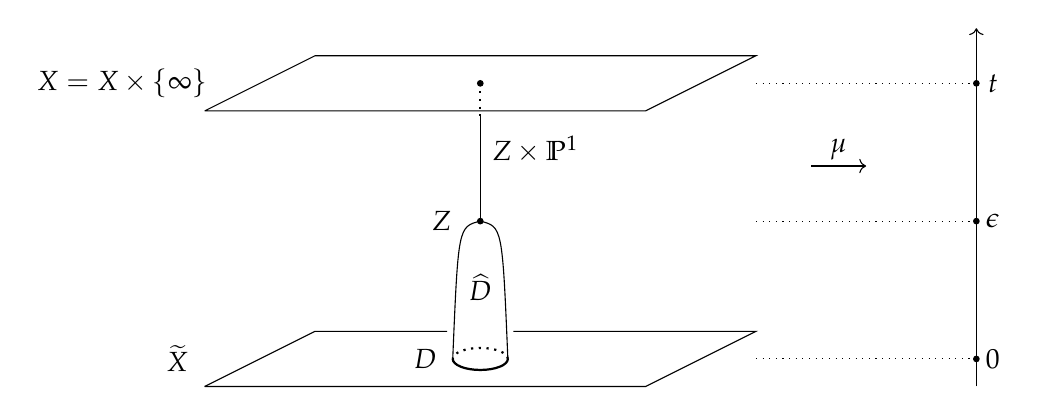
\begin{tikzpicture}[x=0.7cm, y=0.7cm]
\draw (0,5) -- (8,5) -- (10,6) -- (2,6) -- (0,5);
\draw (0,0) -- (8,0) -- (10,1) -- (5.6,1); 
\draw (4.4,1) -- (2,1) -- (0,0);
\filldraw (5,5.5) circle [radius=0.05]; 
\draw[thick, dotted] (5,5.5) -- (5,4.9); 
\draw (5,4.9) -- (5,3); 
\filldraw (5,3) circle [radius =0.05]; 
\draw[thick,dotted] (5.5,0.5) arc [x radius = 0.5, y radius =0.2, start angle=0, end angle =180];
\draw[thick] (4.5,0.5) arc [x radius =0.5, y radius =0.2, start angle =180, end angle = 360]; 
\draw (5,3) .. controls (4.6,2.9) .. (4.5,0.5) ;
\draw (5,3) .. controls (5.4,2.9) .. (5.5,0.5) ;
\draw (-0.5,0.5) node {$\wt{X}$}; 
\draw (-1.5,5.5) node {$X= X\times \{\infty\}$}; 
\draw (4,0.5) node {$D$}; 
\draw (5,1.8) node {$\wh{D}$}; 
\draw (4.3,3) node {$Z$}; 
\draw (6,4.3) node {$Z\times \P^1$}; 
\draw[->] (14,0)--(14,6.5); 
\filldraw (14,5.5) circle [radius=0.05]; 
\filldraw (14,3) circle [radius =0.05]; 
\filldraw (14,0.5) circle [radius =0.05]; 
\draw (14.3,5.5) node {$t$}; 
\draw (14.3,3) node {$\epsilon$}; 
\draw (14.3,0.5) node {$0$}; 
% \draw (14.4,6.5) node {$\mu$};
\draw[dotted] (10,5.5) -- (14,5.5); 
\draw[dotted] (10,3) -- (14,3); 
\draw[dotted] (10,0.5) -- (14,0.5); 
\draw[->] (11,4) -- (12,4); 
\draw (11.5,4.3) node {$\mu$}; 
\end{tikzpicture} 
\caption{$W = \Bl_{Z\times \{0\}} (X\times \P^1)$ and a moment map $\mu \colon W\to \R$}
\label{fig:W}
\end{figure} 

The fixed locus of the $\C^*$-action is given by
\[ W^{\C^*} = X \sqcup \wt{X} \sqcup Z. \]
We can also see that
\begin{align*} 
    N_T^1(W) &= \wh{\varphi}^* N_T^1(X \times \P^1) \oplus \Z[\wt{D}]  \\
    &\cong N^1(X) \oplus \Z^3 \ni (\omega, t, \ep, a).
\end{align*}
Note here that
\[ N_T^1(X \times \P^1) = \on{pr}_1^* N^1(X) \oplus \Z[X] \oplus \Z \lambda, \]
so a general class in $N_1^T(W)$ can be written as
\[ \wh{\varphi}^* \on{pr}_1^* \omega + t [X] - \ep [\wh{D}] + a \cdot \lambda. \]
The dual notion is the group of $1$-cycles, which is given by
\[ N_1^T(W) \cong N_1(X) \oplus \Z^3 \ni (d, k, \ell, m) \eqqcolon \beta, \]
whose Novikov variable is
\[ Q^d x^k y^{\ell} S^m. \]
Note that
\[ [X] \cdot \beta = k, \qquad -[\wh{D}] \cdot \beta = \ell. \]
The effective curve classes are those which are equivariant, so they either lie in the fixed loci or are $1$-dimensional orbits. There are classes $C_1$ lying entirely inside $X$, classes $C_2$, which are $x \times \P^1$ for $x \notin Z$, classes $C_3 \subset Z \times \P^1$, and classes $C_4 \subset \wh{D}$. The corresponding Novikov variables are $Q^d, x, xy^{-1}$, and $y$, respectively.

\begin{lem}
    The monoid of effective curve classes is generated by $C_1, C_2, C_3, C_4, S$.
\end{lem}

\begin{exm}
    Let $X = \P^1 \times \P^1$ and $Z = (0,0)$. Then a toric diagram for $W$ with $C_1, C_2, C_3, C_4$ is given in~\Cref{fig:toric}.
    \begin{figure}[htpb]
    \begin{center}
    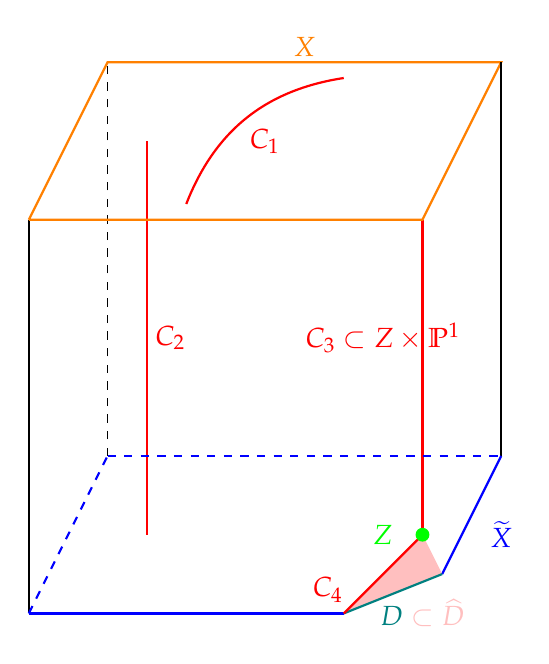
\begin{tikzpicture}[scale=1]
        \draw[thick] (0,0) -- (0,5);
        \draw[dashed] (1,2) -- (1,7);
        \draw[dashed, thick, blue] (0,0) -- (1,2);
        \draw[thick,red] (5,1) -- (5,5);
        \draw[thick,red] (1.5,1) -- (1.5,6);
        \draw[thick,orange] (0,5) -- (1,7) -- (6,7) -- (5,5) -- (0,5);
        \draw[thick] (6,7) -- (6,2);
        \draw[dashed,thick,blue] (1,2) -- (6,2);
        \draw[thick,blue] (0,0) -- (4,0);
        \draw[thick,blue] (6,2) -- (5.25,0.5);
        \fill[pink] (4,0) -- (5,1) -- (5.25,0.5) -- cycle;
        \draw[thick,teal] (5.25,0.5) -- (4,0);
        \draw[thick,red] (2,5.2) to [bend left=30] (4,6.8);
        \draw[thick,red] (4,0) -- (5,1);
        \node[text=blue] at (6,1) {$\wt{X}$};
        \node[text=orange] at (3.5,7.2) {$X$};
        \node[circle,fill=green,minimum size=5pt,inner sep=0pt] at (5,1) {};
        \node[text=green] at (4.5,1) {$Z$};
        \node[text=pink] at (5,0) {$\textcolor{teal}{D} \subset \wh{D}$};
        \node[text=red] at (4.5,3.5) {$C_3 \subset Z \times \P^1$};
        \node[text=red] at (3,6) {$C_1$};
        \node[text=red] at (1.8, 3.5) {$C_2$}; 
        \node[text=red] at (3.8, 0.3) {$C_4$};
    \end{tikzpicture}
    \end{center}
    \caption{Toric diagram of $W$ for $X = \P^1 \times \P^1$ and $Z = (0,0)$ with curve classes $C_1, C_2, C_3, C_4$.}%
    \label{fig:toric}
    \end{figure}
\end{exm}


The $T$-ample cone $C_T(W)$ of $W$ is the dual to the cone of effective curve classes. Then $\wh{\omega} \in C_T(W)$ if the set of $\wh{\omega}$-stable points under the $\C^*$-action is nonempty. Then there is a decomposition
\[ \ol{C_T(W)} = \ol{C}_X \cup \ol{C}_{\wt{X}} \]
into pieces where the GIT quotient
\[ W \sslash_{\wh{\omega}} T \cong X \text{ or } \wt{X}, \]
respectively. The stable points are
\begin{itemize}
    \item For $\wh{\omega} \in C_X$, the stable points are $X \times \C^*$;
    \item For $\wh{\omega} \in C_{\wt{X}}$, the stable points are $\mc{O}_{\wt{X}}(-\wh{D}) \setminus \wh{X}$.
\end{itemize}

The dual cones $C_X^{\vee}$ and $C_{\wt{X}}^{\vee}$ correspond to embeddings of the effective cones of $X$ and $\wt{X}$, respectively, into the effective cone of $W$ as in~\Cref{fig:Mori_cones}.

\begin{figure}[htpb]
\centering 
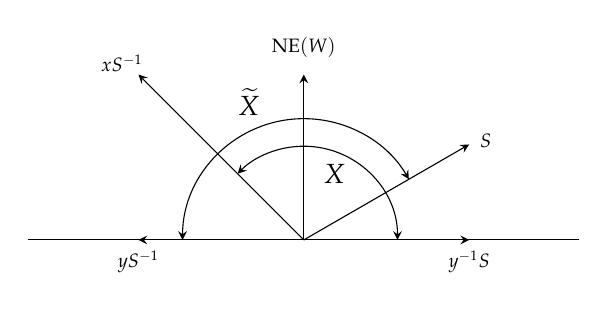
\begin{tikzpicture}[>=stealth, x=0.7cm, y=0.7cm]
\draw (-5,0) -- (5,0); 
\draw[->] (0,0) -- (-3,0); 
\draw[->] (0,0) -- (3,0);
\draw[->] (0,0) -- (0,3); 
\draw[->] (0,0) -- (3,1.732);
\draw[->] (0,0) --(-3,3);  
\draw (0,3.5) node {\scriptsize $\on{NE}(W)$}; 
\draw (-3,-0.4) node {\scriptsize $y S^{-1}$}; 
\draw (3,-0.4) node {\scriptsize $y^{-1} S$}; 
\draw (-3.3,3.2) node {\scriptsize $x S^{-1}$}; 
\draw (3.3,1.8) node {\scriptsize $S$};

\draw [<->] (-2.2,0) arc[start angle =  180, end angle = 30, radius = 2.2]; 
\draw [<->] (1.7,0) arc[start angle =0, end angle = 135, radius = 1.7]; 
\draw (-1,2.5) node {$\wt{X}$}; 
\draw (0.55,1.2) node {$X$}; 
\end{tikzpicture} 

\caption{A schematic picture of the cones $C_X^{ \vee }$ and $C_{ \wt{X} }^{ \vee }$ in $N_1^T(W)$.} 
\label{fig:Mori_cones} 
\end{figure} 

Recall the \textit{Kirwan map}
\begin{align*}
    \kappa_Y &\colon H_T^*(W) \twoheadrightarrow H_T^*(W^s) = H^*(Y) \\
    \kappa_Y^* &\colon \on{NE}_{\N}(Y) \to N_1^T(W),
\end{align*}
where $Y$ is either $X$ or $\wt{X}$.

Now consider the equivariant quantum $D$-module
\[ QDM_T(W) = H_T^*(W)[z] \llbracket \mc{Q}, \theta \rrbracket \]
endowed with the quantum connection and the action of the shift operators
\[ \wh{\mb{S}}_{\beta}(\theta), \qquad \beta \in N_1^T(W) \cong N_1(X) \oplus \Z^3, \]
which are defined by
\[ \wh{\mb{S}}^{\beta}(\theta) = Q^d x^k y^{\ell} \mb{S}(\theta)^m, \]
where $\beta$ is identified with $(d, k, \ell, m)$ under the factorization $N_1(X) \oplus \Z^3$.

We can obtain the quantum $D$-modules for $X$ and $\wt{X}$ from the equivariant quantum $D$-module of $W$ by taking affine charts and completing. Here, we think of $\QDM_T(W)$ as a global K\"ahler moduli space.
\begin{figure}[htpb] 
\centering 
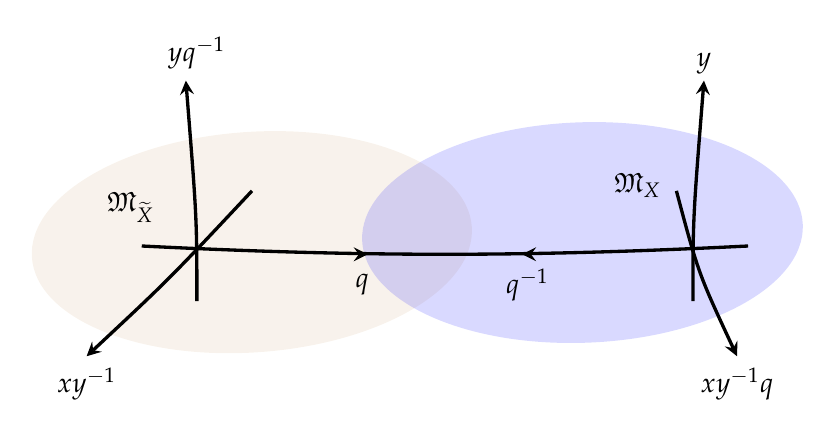
\begin{tikzpicture}[x=0.7cm, y=0.7cm, >=stealth]
\fill[brown, rotate=4,opacity=0.1] (1,0) ellipse [x radius =4, y radius =2];
\fill[blue, rotate =2, opacity=0.15] (7,0) ellipse [x radius=4, y radius = 2]; 

\draw[very thick] (-1,0).. controls (3,-0.2) and (6,-0.2) .. (10,0); 
\draw[very thick, ->] (0,-1) .. controls (0,0.5) .. (-0.2,3); 
\draw[very thick, ->] (1,1) .. controls (-0.5, -0.6) .. (-2,-2); 
\draw[very thick,->] (3,-0.15)--(3.1,-0.15); 

\draw[very thick,->] (9,-1) .. controls (9,0.5) .. (9.2,3); 
\draw[very thick,->] (8.7,1) .. controls (9.1,-0.5) .. (9.8,-2);
\draw[very thick,->] (6,-0.15) -- (5.9,-0.15); 

\draw (3,-0.7) node {$q$}; 
\draw (-2,-2.5) node {$xy^{-1}$}; 
\draw (0,3.5) node {$y q^{-1}$}; 

\draw (6,-0.7) node {$q^{-1}$}; 
\draw (9.8,-2.5) node {$xy^{-1} q$}; 
\draw (9.2,3.3) node {$y$}; 

\draw (-1.2,0.7) node {$\mf{M}_{ \wt{X} }$}; 
\draw (8,1.1) node {$\mf{M}_{X}$}; 
\end{tikzpicture} 
\caption{Global K\"ahler moduli space associated with $\QDM_T(W)$. See also Figure \ref{fig:Mori_cones}. }
\label{fig:global}  
\end{figure} 

\subsection{Fourier transforms}%
\label{sub:Fourier transforms}

To construct the map in~\Cref{thm:blowup}, Iritani uses both the discrete and continuous Fourier transforms. For $f \in \mc{H}_W$, the discrete Fourier transform is given by
\[ F_Y(f) \coloneqq \sum_{k \in \Z} S^k \kappa_Y(\mc{S}^{-k} f) \in \mc{H}_Y^{\mr{ext}}. \]
The continuous Fourier transform for $Z \in \pi_0(W^T)$ is given by sending $f \in \mc{H}_W$ to the element of $\mc{H}_Z$ given by the formal asymptotic expansion of
\[ \int e^{\lambda \log \frac{S}{z}} \Delta_Z^{-1} f|_{Z} \d \lambda. \]

\begin{rmk}
    We can think of $X$ and $\wt{X}$ either as fixed components $X, \wt{X} \in \pi_0(W^T)$ (corresponding to the continuous Fourier transform) or as GIT quotients $W \sslash_{\wh{\omega}} T$, corresponding to the discrete Fourier transform. These are in fact equal up to a factor.

    Note that $Z$ is not a GIT quotient of $W$, but is a fixed component, so there is a continuous Fourier transform to $W$. In total, we have three morphisms
    \begin{equation*}
    \begin{tikzcd}
        & \QDM(\wt{X}) \\
        \QDM_T(W) \ar{ur}{\cong} \ar{r} \ar{dr}{r-1} & \QDM(X) \\
        & \QDM(Z).
    \end{tikzcd}
    \end{equation*}
\end{rmk}

\section{Fourier analysis for blowups (Sam, Mar 21)}%
\label{sec:Fourier analysis for blowups}

In this section, denote the Chern roots of $\mc{N}_{Z/X}$ by $\ep_1, \ldots, \ep_r$. 

\subsection{Extended Kirwan maps}%
\label{sub:Extended Kirwan maps}

We will begin by describing the Kirwan maps in coordinates. On $H^2_T(W)$, we have
\begin{align*}
    \kappa_X \colon & \wh{\varphi}^* \on{pr}_1^* \alpha \mapsto \alpha \\
    & [X] \mapsto 0 \\
    & -[\wh{D}] \mapsto 0 \\
    & \lambda \mapsto 0 
\end{align*}
for $Y = X$
\begin{align*}
    \kappa_{\wt{X}} \colon & \wh{\varphi}^* \on{pr}_1^* \alpha \mapsto \varphi^* \alpha \\
    & [X] \mapsto 0 \\
    & -[\wh{D}] \mapsto -[D] \\
    & \lambda \mapsto [D]
\end{align*}
for $Y = \wt{X}$. The dual Kirwan maps on $N_1(Y)$ are given by
\begin{align*}
    \kappa_X^* \colon & N_1(X) \to N_1^T(W) \cong N_1(X) \oplus \Z \lambda^{\vee} \oplus \Z[X]^{\vee} \oplus \Z(-[\wh{D}])^{\vee} \\
    & d \mapsto (d,0,0,0) \\
    \kappa_{\wt{X}}^* \colon & N_1(\wt{X}) \to N_1^T(W) \cong N_1(X) \oplus \Z \lambda^{\vee} \oplus \Z[X]^{\vee} \oplus \Z(-[\wh{D}])^{\vee} \\
    & \wt{d} \mapsto (\varphi_* \wt{d},0,-[D] \cdot \wt{d},[D] \cdot \wt{d})
\end{align*}
when $Y=X$ and $Y=\wt{X}$, respectively. It may appear that we don't see the equivariant parameters in the dual Kirwan map, but we will fix this.

\begin{defn}
    The \textit{extended Givental space} is
    \[ \mc{H}_Y^{\mr{ext}} \coloneqq H^*(Y)[z^{\pm}] \llbracket C_{Y,N}^{\vee} \rrbracket, \]
    which is a base change of $\mc{H}_Y$.
\end{defn}

The shift operators on $\mc{H}_W^{\mr{rat}} = H_{\mr{loc}}^*(W)[Z^{\pm}]\llbracket Q \rrbracket$ are now given by
\[ \mc{S} \iota_* (f_X, f_Z, f_{\wt{X}}) = (\mc{S} f|_X, \mc{S}f|_Z, \mc{S} f|_{\wt{X}}),\]
where
\begin{align*}
    \mc{S}^k f_X &= x^k \frac{\prod_{c=-\infty}^0 (-\lambda + cz)}{\prod_{c=-\infty}^k (-\lambda + cz)} e^{-kz \partial_{\lambda}} f_X \\
    \mc{S}^k f_Z &= y^k \frac{\prod_{c=-\infty}^0 \prod_{i=1}^r (\ep_i-\lambda + cz) \prod_{c=-\infty}^0 (\lambda + cz)}{\prod_{c=-\infty}^k \prod_{i=1}^r (\ep_i-\lambda + cz) \prod_{c=-\infty}^k (\lambda + cz)} e^{-kz \partial_{\lambda}} f_X \\
    \mc{S}^k f_{\wt{X}} &= \frac{\prod_{c=-\infty}^0 ([D] + \lambda + cz)}{\prod_{c=-\infty}^k ([D] + \lambda + cz)} e^{-kz \partial_{\lambda}} f_{\wt{X}}.
\end{align*}

\subsection{Discrete Fourier transform}%
\label{sub:Discrete Fourier transform blowup}

We are now able to make the following definition.

\begin{defn}
    The \textit{discrete Fourier transform} is
    \[ F_Y \colon \mc{H}_W^{\mr{rat}}[Q^{-1}] \dashrightarrow \mc{H}_Y^{\mr{ext}}[Q^{-1}], \]
    defined by
    \[ F_Y(f) = \sum_{k \in \Z} S^k \kappa_Y (\mc{S}^{-k} f). \]
\end{defn}

Because we invert the equivariant parameters, this may not necessarily be well-defined. However, we do have the following result.

\begin{prop}
    The discrete Fourier transform $F_Y$ is well-defined on tangent spaces to $\mc{L}_W$.
\end{prop}

To prove this result, we need various ingredients:
\begin{enumerate}
    \item Some regularity at $\lambda = 0$, which follows from properness;
    \item Not needing arbitrarily high powers of $Q^{-1}$ (landing in the target).
\end{enumerate}

As in the case of projective bundles, the shift operators satisfy various nice properties. For example, because
\[ [\lambda, \mc{S}^k] = z^k \mc{S}, \]
we obtain the formulae
\begin{align*}
    F_Y(\mc{S}^{\ell} f) &= S^{\ell} F_Y(f) \\
    F_Y(\xi f) &= (z \xi Q \partial_Q + \kappa_Y(\xi)) F_Y(f)
\end{align*}
for any $\xi \in H_2^T(W)$.

\subsection{Continuous Fourier transform}%
\label{sub:Continuous Fourier transform blowup}

Let $F \in \ab\{X, \wt{X}, Z\}$ be a fixed component in $W^T$. Denote the Chern roots of $\mc{N}_{F/W}$ by $\rho_1, \ldots, \rho_n$. Now define
\[ G_F \coloneqq \prod_{\rho} \frac{1}{\sqrt{- 2\pi z}} (-z)^{-\frac{\rho}{z}} \Gamma\ab(\frac{-\rho}{z}). \]
More specifically, for each individual fixed component, we have
\begin{align*}
    G_X &= \frac{1}{-2\pi z}(-z)^{\frac{\lambda}{z}} \Gamma \ab(\frac{\lambda}{z}) \\
    G_Z &= \frac{1}{\sqrt{-2\pi z}^{r+1}} (-z)^{-\frac{\lambda}{z}} \Gamma\ab(\frac{-\lambda}{z}) \prod_{i=1}^r (-z)^{\frac{\lambda - \ep_i}{z}} \Gamma\ab(\frac{\lambda - \ep_i}{z}) \\
    G_{\wt{X}} &= \frac{1}{\sqrt{-2\pi z}}(z)^{\frac{[D]-\lambda}{z}} \Gamma \ab(\frac{[D]-\lambda}{z}).
\end{align*}
This $G_F$ actually intertwines all $\wh{\mc{S}}^{\beta}$, which are defined for all
\[ \beta \in N_1^T(W) \to H_2(BT) \ni \ol{\beta}. \]
Given $F$, we have
\[ \sigma_k(F) \in N_1(E_k) \to N_1^T(W), \]
which are obtained by section classes on $E_k$ as in~\Cref{fig:toricEk}. Now $G_F$ satisfies the equation
\[ G_F (\wh{\mc{S}}^{\beta}f)_F = (Q^{\beta + \sigma_F(-\ol{\beta})} e^{-z \ol{\beta} \partial_{\lambda}}) G_F f, \]
which follows from the same argument as in the projective bundle case.

\begin{figure}[htpb]
\begin{center}
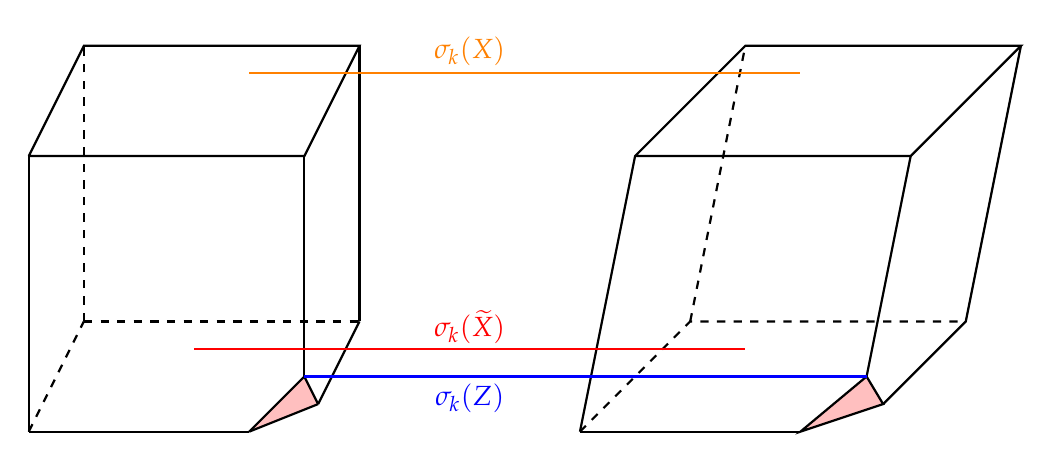
\begin{tikzpicture}[scale=0.7]
    \draw[thick] (0,0) -- (0,5);
    \draw[dashed, thick] (1,2) -- (1,7);
    \draw[dashed, thick] (0,0) -- (1,2);
    \draw[thick] (5,1) -- (5,5);
    % \draw[thick] (1.5,1) -- (1.5,6);
    \draw[thick] (0,5) -- (1,7) -- (6,7) -- (5,5) -- (0,5);
    \draw[thick] (6,7) -- (6,2);
    \draw[dashed,thick] (1,2) -- (6,2);
    \draw[thick] (0,0) -- (4,0);
    \draw[thick] (6,2) -- (5.25,0.5);
    \fill[pink] (4,0) -- (5,1) -- (5.25,0.5) -- cycle;
    \draw[thick] (5.25,0.5) -- (4,0);
    \draw[thick] (4,0) -- (5,1);
    \draw[thick] (5.25,0.5) -- (5,1);
    % \node[circle,fill=blue,minimum size=5pt,inner sep=0pt] at (5,1) {};
    \draw[thick] (10,0) -- (11,5) -- (13,7) -- (18,7) -- (16,5) -- (11,5);
    \draw[dashed,thick] (10,0) -- (12,2) -- (17,2);
    \draw[dashed,thick] (12,2) -- (13,7);
    \draw[thick] (18,7) -- (17,2) -- (15.5,0.5);
    \draw[thick] (10,0) -- (14,0);
    \fill[pink] (14,0) -- (15.5,0.5) -- (15.2,1) -- cycle;
    \draw[thick] (14,0) -- (15.5,0.5) -- (15.2,1) -- cycle;
    \draw[thick] (16,5) -- (15.2,1);
    % \node[circle,fill=blue,minimum size=5pt,inner sep=0pt] at (15.2,1) {};
    \draw[blue, thick] (5,1) -- (15.2,1);
    \node[text=blue] at (8,0.6) {$\sigma_k(Z)$};
    \draw[red, thick] (3,1.5) -- (13,1.5);
    \node[text=red] at (8,1.9) {$\sigma_k(\wt{X})$};
    \draw[orange, thick] (4,6.5) -- (14,6.5);
    \node[text=orange] at (8,6.9) {$\sigma_k(X)$};
\end{tikzpicture}
\end{center}
\caption{Toric diagram of $E_k$ when $X, Z$ are as in~\Cref{fig:toric}.}%
\label{fig:toricEk}
\end{figure}

We are now able to describe the continuous Fourier transform formally as an integral which has the same properties as the discrete one. Define
\[ \mc{FT}^{\infty} \colon f \mapsto \int e^{\lambda \log \frac{S_f}{z}} G_F f_F \d \lambda, \]
where $S_F = \sigma_1(F)$. Formally, we see that
\begin{align*}
    \mc{FT}^{\infty}(\wh{\mc{S}}^{\beta} f) &= \int e^{\lambda \log \frac{S_F}{z}} Q^{\beta + \sigma_1(-\ol{\beta})} e^{z \ol{\beta} \log \frac{S_F}{z}} G_F f_F \d \lambda \\
    &= \wh{\mc{S}^{\beta}} \mc{FT}^{\infty}(f),
\end{align*}
which suggests that this is the right object to study the asymptotics of. Recall the Stirling approximation
\begin{align*}
    \log G_F &\asymp \sum_{\rho_i}- \frac{\rho_i \log \rho_i - \rho_i}{z} - \frac{1}{2}\log \rho_i - \sum_{n=2}^{\infty} \frac{B_n}{n(n-1)} \ab(\frac{z}{\rho_i})^{n-1}, \\
    &= \sum_{\alpha \in \mr{wts}(\mc{N}_{F/W})} \ab(- r_{\alpha} \frac{\alpha \log \alpha - \alpha}{z} - \log \Delta_{\alpha}),
\end{align*}
where we have the decomposition
\[ \mc{N}_{F/W} = \bigoplus_{\alpha} \mc{N}^{\alpha}, \]
$\rho_{\alpha} = c_1(\mc{N}^{\alpha})$ is the first Chern class, $r_{\alpha} = \on{rk} \mc{N}^{\alpha}$, and $\Delta_{\alpha}$ is the quantum Riemann-Roch operator. We now obtain
\begin{align*}
    \mc{FT}^{\infty} &\asymp \int e^{\frac{\lambda \log S_F - \sum_{\alpha} r_{\alpha}(\alpha \log \alpha - \alpha)}{z}} \prod_{\alpha} \Delta_{\alpha}^{-1} f_F \d \lambda.
\end{align*}
We have a critical point
\[ \lambda_0 = S_F^{\frac{1}{c}} \prod_{\alpha} w_{\alpha}^{-r_{\alpha} \frac{w_{\alpha}}{c_F}}, \]
where
\[ c_F = \begin{cases}
    -1 & F=X \\
    1 & F=\wt{X} \\
    -(r-1) & F=Z.
\end{cases}
\]
Also, for $j = 0, \ldots, \abs{c_F}-1$, we have critical points
\[ \lambda_j = e^{\frac{2\pi \sqrt{-1} j}{c_F}} \lambda_0. \]

\begin{defn}
    The \textit{continuous Fourier transform} is given by the asymptotic expansion
    \[ \int e^{\lambda \log \frac{S_F}{z}} G_F f_F \d \lambda \asymp \sqrt{2\pi z} e^{r\frac{\lambda_j}{z}} \mc{F}_{F,j}(f), \]
    where we take the asymptotics as $z \to 0$ and substitute
    \[ \lambda = \lambda_j \exp\ab(\frac{u}{\sqrt{c \lambda_j}}) \]
    and expand in $u$-powers as $u \to 0$.
\end{defn}

Via taking a formal asymptotic analysis of what we did before, we have
\begin{prop}\leavevmode
    \begin{enumerate}
        \item The continuous Fourier transform intertwines the shift operators as
            \[ \mc{F}_{F,j}(\wh{\mc{S}}^{\beta} f) = \wh{S}^{\beta} \mc{F}_{F,j}(f); \]
        \item The continuous Fourier transform intertwines the equivariant parameter via
            \[ \mc{F}_{F,j}(\lambda f) = (z S + \lambda_j) \mc{F}_{F,j}(f). \]
        \item There is a similar property for the Euler vector field.
    \end{enumerate}
\end{prop}

Now let
\[ \wh{J}_{F,j}^{\mr{tw}} = \mc{F}_{F,j} (\iota_* J_F^{\mr{tw}}(t)). \]

\begin{prop}\label{prop:twisted}
    There exists 
    \[ \tau(t) \in H^*(F) \llbracket S_F^{-\frac{1}{c}}, Q_F S^{-\frac{\rho_F}{c}}, tS_F^{\frac{*}{c}} \rrbracket \]
    and
    \[ v(t) \in H^*(F) [z] \llbracket S_F^{-\frac{1}{c}}, Q_F S^{-\frac{\rho_F}{c}}, tS_F^{\frac{*}{c}} \rrbracket \]
    such that 
    \[ \wh{J}_{F,j}^{\mr{tw}} = S_F^{-\frac{\rho_F}{cz}} M_F(\tau(t) Q_F S_F^{-\frac{\rho_F}{cz}}) v. \]
\end{prop}

In other words, we can recover $\QDM_F$ from $\mc{F}_{F,j}$ after a change of basis and an \'etale cover of the K\"ahler moduli space.

\begin{prop}
    The discrete and continuous Fourier transforms agree for $Y \in \ab\{X, \wt{X} \}$. In other words, we have
    \[ e^{S_Y^{\frac{1}{c_Y}}} \mc{F}_{Y,0}(f) = c_Y^{-1} S_Y^{-\frac{\rho_Y}{c_Y z}} F_Y(f). \]
\end{prop}



\section{Decomposition (Sam, Mar 28)}%
\label{sec:Decomposition}

\subsection{A general picture}%
\label{sub:A general picture}

We begin by stating some general conjectures that the blowup result fits into.

\begin{conj}[Dubrovin]
    Let $X$ be smooth and projective. If there exists a semiorthogonal decomposition
    \[ D^b(X) = \ab<D^b(X_1), \ldots, D^b(X_n)>, \]
    then there is a decomposition
    \[ \QDM(X) = \bigoplus_i \QDM(X_i). \]
    More specifically, if $X$ admits a full exceptional collection, $\QDM(X)$ can be extended to $\mc{O}^{\mr{an}}\llbracket z \rrbracket$. In addition the Gram matrix of the pairing $\chi(-,-)$ on $K(X)$ is recovered as the Stokes matrix
    \[ S = \Phi_{\on{arg} z \in (-\pi, 0+\ep)} \Phi^{-1}_{\on{arg} z \in (0,\pi)} \]
    of flat sections of the irregular connection
    \[ z \partial_z + \frac{1}{z}E_X \star_{\tau} + \mu_X. \]
\end{conj}

On the level of derived categories, we have a decomposition
\[ D^b(\wt{X}) = \ab< D^b(X), D^b(Z)_0, \ldots, D^b(Z)_{r-2}>, \]
so we expect a decomposition
\[ \QDM(\wt{X}) = \bigoplus_{\mu \in \Spec(E_{\wt{X}} \star_{\tau})} \QDM(\wt{X})_{\mu}. \]
In the limit $Q\tau \to 0$, we obtain $\QDM(X)$ at $\mu = 0$ and $r-1$ copies of $\QDM(Z)$ at roots of unity. The shift away from $\mu = 0$ will correspond to the shift of saddle points in the Fourier transform.

In the equivariant setting, we have semiorthogonal decompositions
\[ D^b_T(W) = \ab<D^b(W\sslash_{\theta} T), \ldots>. \]
We then expect
\begin{conj}
    Setting $W \sslash_{\theta} T \eqqcolon Y$, then
    \[ I \coloneqq \sum_{\beta} \kappa_Y(\wh{S}^{-\beta} J_W(\tau)) \wh{S}^{\beta} \]
    lies on the Lagrangian cone of $Y$.
\end{conj}


\subsection{Decomposition of the quantum $D$-module}%
\label{sub:Decomposition of the quantum D module}

First, we would like to give a more precise formulae for the quantities appearing in~\Cref{prop:twisted}. First, $\tau$ is given by
\[ \tau|_{Q=0} = h_{F,j} + \cdots, \]
where
\[ h_{F,j} = 2 \pi i j \frac{c_1(N_{F/W})}{C_F} + \sum_{\alpha} \ab(\on{rk}_{\alpha} w_{\alpha} \frac{c_1(N_{F/W})}{c_F} - c_1(N_{F/W}^{\alpha})). \]
Then we have
\[ v|_{Q=0} = q_{F,j}(1+ \cdots), \]
where
\[ q_{F,j} = \sqrt{c_F^{-1} \lambda_j} \prod_{\alpha} (w_{\alpha \lambda_j})^{\frac{\on{rk}_{\alpha}}{2}} \]
for $\lambda_j = e^{\frac{1\pi i j}{c_F}} \lambda_0$.

For $X, \wt{X}$, the continuous Fourier transform $\mc{F}_{F,j}$ intertwines $S^{\beta}$ and $\lambda$ with $\xi S \pdv{}{S}$ and $E_W^T \star_{\tau} + \mu_W$ with $E_{\wt{X}} \star_{\tau} + \mu_X + \frac{1}{2}$. On the other hand, for $F=Z$, the critical points are different, so there is a shift in $\lambda$. For example, we have
\[ \mc{F}_{F,j}(\lambda f) = \ab(z S \pdv{}{S} + \lambda_j) \mc{F}_{F,f}(f) \]
because the integral satisfies the formula
\[ z S \pdv{}{S} \int e^{\log \frac{S_F}{z}(\lambda - \lambda_j)} f G \d \lambda = \int (\lambda - \lambda_j) e^{\log \frac{S_F}{z} (\lambda - \lambda_j)} f G \d \lambda. \]
A similar argument yields
\[ \mc{F}_{F,j} \ab( \ab(z \partial_z + \mu_Z + \frac{1}{2}) f) = (z \partial_z + z^{-1}(c_1(F) + c_F \lambda_j + \mu_F)) \mc{F}_{F,j}(f). \]

We next need a space on which to compare $\QDM(X)$, $\QDM(\wt{X})$, and $\QDM_T(W)$ via the dual Kirwan maps. Define
\[ \QDM(Y)^{\on{ext}} \coloneqq \QDM(Y) \otimes \C \llbracket C_{Y, \N}^{\vee} \rrbracket \]
and extend $\nabla$ trivially on $C_{Y,\N}^{\vee}$. As in~\Cref{fig:global}, we have $\mf{M}_{\wt{X}}$ and $\mf{M}_X$, but we also need
\[ \mf{M}_0 = \on{Spf} \C[z] \llbracket \on{NE}_{\N}^T(W) \rrbracket \llbracket \theta \rrbracket. \]
The three charts can be compared on the chart
\[ \mf{U} = \on{Spf} \C[z] \llbracket \on{NE}_{\N}^T(W) \rrbracket \llbracket \theta \rrbracket \llparenthesis q^{-\frac{1}{s}} \rrparenthesis. \]
The comparison of the effective cones of curves is given in~\Cref{fig:Mori_cones}.

The comparison also requires a completion and localization of $\QDM_T(W)$. In order to compare with $\QDM(\wt{X})$ we need the action of extended shift operators $\mathbb{S}^{\beta}$. Define
\[ \QDM_T(W)_{\wt{X}} \coloneqq \C[C_{\wt{X}, \N}^{\vee}] \cdot \QDM_T(W) \subset \QDM_T(W) (Q^{-1}). \]
The completion is given by
\[ \wh{\QDM}_T(W)_{\wt{X}} = \QDM_T(W) \llbracket S, yS^{-1} \rrbracket. \]

Now let
\begin{align*}
    \tau(\theta) &= x S + \cdots \\
    v(\theta) &= 1 + \cdots \\
    \wt{\tau}(\theta) &= S + \cdots \\
    \wt{v}(\theta) &= 1 + \cdots
\end{align*}
such that
\begin{align*}
    F_X(J_w(\theta)) &= M_X(\tau(\theta)) v(\theta) \\
    F_{\wt{X}}(J_w(\theta)) &= M_{\wt{X}}(\wt{\tau}(\theta)) \wt{v}(\theta).
\end{align*}
By taking derivatives $\partial_{\theta^{ik}}$, the Fourier transform is lifted to a map of quantum $D$-modules.

\begin{thm}
    There is an isomorphism
    \[ \wh{\on{FT}}_{\wt{X}} \colon \wh{\QDM}_T(W)_{\wt{X}} \to \wt{\tau}^* \QDM(\wt{X})^{\on{ext}} \]
    and a projection
    \[ \wh{\on{FT}}_X \colon \wh{\QDM}_T(W)_{\wt{X}} \to \tau^* \QDM(X)^{\on{ext}}. \]
    They intertwine the quantum connection and the pairing up to a $\frac{1}{2}$ shift in $\mu$.
\end{thm}

These extend to the completions, but we will not prove this here.

For $F=Z$ and any $j$, there are coordinates
\begin{align*}
    \sigma_j(\theta) &= h_{Z,j} + \cdots \\
    u_jj(\theta) ^= q_{Z,j} + \cdots
\end{align*}
such that
\[ q^{\frac{c_1(N_{Z/W})}{(r-1)z}} \mc{F}_{Z,j}(J_w(\theta)) = M(\sigma_j(\theta))u_j(\theta). \]

\begin{thm}
    There are projections
    \[ \wh{\on{FT}}_{Z,j} \colon \wh{\QDM}_T(W)_{\wt{X}} \to \sigma_j^* \QDM(Z)^{\mr{ext,loc}} \]
    which intertwine $\lambda$ with $z \nabla_{S \partial_S} + \lambda_j$ and $z \nabla_{\xi Q \partial_Z}$ with $z \nabla_{\wh{S} \partial_{\wh{S}}} + \iota_{\mr{pt}}^* \xi |_{\lambda = \lambda_i}$. Here, $\QDM(Z)^{\mr{ext,loc}}$ is defined by the extension
    \[ \C[z] \llbracket Q_Z, \theta \rrbracket \to \C[z] \llbracket q^{-\frac{1}{s}} \rrbracket \llbracket Q, \theta \rrbracket \qquad Q_Z^d \mapsto Q^{(\iota_Z)_* d} q^{-\frac{c_1(N_{Z/W})\cdot d}{r-1}}. \]
\end{thm}

We will now shift our variables in order to make our comparison. Let
\[ \varsigma_j(\theta) = \sigma_j(\theta) - (r-1)\lambda_j. \]
Then
\[ \wh{\on{FT}}_{Z,j}^{\varsigma} \colon \wh{\QDM}_T(W) \to \varsigma_j^* \QDM(Z)^{\mr{ext,loc}} \]
intertwines the quantum connections up to a $\frac{1}{2}$ shift in $\mu_Z$. Combining the Fourier transforms for the different fixed loci, we obtain

\begin{thm}[Main theorem]\label{thm:main}
    The diagram
    \begin{equation*}
    \begin{tikzcd}
        & & \tau^* \QDM(X)^{\mr{ext}} \\
        \wt{\tau}^* \QDM(\wt{X})^{\mr{ext}} \ar{r}{\wh{\on{FT}}_X^{-1}} & \wh{\QDM}_T(W)_{\wt{X}} \ar{ur}{\wh{\on{FT}}_X} \ar{dr}{\bigoplus_j \wh{\on{FT}}_{Z,j}}  \\
        & & \bigoplus_j \varsigma_j^* \QDM(Z)^{\mr{ext,loc}}
    \end{tikzcd}
    \end{equation*}
    induces an isomorphism
    \[ \wt{\tau}^* \QDM(\wt{X})^{\mr{ext}} \simeq \tau^* \QDM(X)^{\mr{ext}} \oplus \bigoplus_j \varsigma_j^* \QDM(Z)^{\mr{ext,loc}} \]
    over $\mf{U}$ that intertwines the quantum connections and Poincar\'e pairings.
\end{thm}







\end{document} 

%%% Local Variables:
%%% mode: latex
%%% TeX-master: t
%%% End:
